\documentclass[
]{jss}

%% recommended packages
\usepackage{orcidlink,thumbpdf,lmodern}

\usepackage[utf8]{inputenc}

\author{
H. Sherry Zhang\\Monash University \And Dianne Cook\\Monash University \AND Ursula Laa\\University of Natural Resources and Life Sciences \AND Nicolas Langrené\\BNU-HKBU United International College \And Patricia Menéndez\\Monash University
}
\title{\pkg{cubble}: An R Package for Organizing and Wrangling Multivariate Spatio-temporal Data}

\Plainauthor{H. Sherry Zhang, Dianne Cook, Ursula Laa, Nicolas Langrené, Patricia Menéndez}
\Plaintitle{cubble: An R Package for Organizing and Wrangling Multivariate Spatio-temporal Data}


\Abstract{
Multivariate spatio-temporal data refers to multiple measurements taken across space and time. For many analyses, spatial and time components can be separately studied: for example, to explore the temporal trend of one variable for a single spatial location, or to model the spatial distribution of one variable at a given time. However for some studies, it is important to analyse different aspects of the spatio-temporal data simultaneouly, like for instance, temporal trends of multiple variables across locations. In order to facilitate the study of different portions or combinations of spatio-temporal data, we introduce a new data structure, \code{cubble}, with a suite of functions enabling easy slicing and dicing on the different components spatio-temporal components. The proposed \code{cubble} structure ensures that all the components of the data are easy to access and manipulate while providing flexibility for data analysis. In addition, \code{cubble} facilitates visual and numerical explorations of the data while easing data wrangling and modelling. The \code{cubble} structure and the functions provided in the \code{cubble} R package equip users with the capability to handle hierarchical spatial and temporal structures. The \code{cubble} structure and the tools implemented in the package are illustrated with different examples of Australian climate data.
}

\Keywords{spatial, temporal, spatio temporal, \proglang{R}, environmental data, exploratory data analysis}
\Plainkeywords{spatial, temporal, spatio temporal, R, environmental data, exploratory data analysis}

%% publication information
%% \Volume{50}
%% \Issue{9}
%% \Month{June}
%% \Year{2012}
%% \Submitdate{}
%% \Acceptdate{2012-06-04}

\Address{
    H. Sherry Zhang\\
    Monash University\\
    21 Chancellors Walk, Clayton VIC 3800 Australia\\
  E-mail: \email{huize.zhang@monash.edu}\\
  
      Dianne Cook\\
    Monash University\\
    21 Chancellors Walk, Clayton VIC 3800 Australia\\
  E-mail: \href{mailto:dicook@monash.edu}{\nolinkurl{dicook@monash.edu}}\\
  
      Ursula Laa\\
    University of Natural Resources and Life Sciences\\
    Gregor-Mendel-Straße 33, 1180 Wien, Austria\\
  E-mail: \href{mailto:ursula.laa@boku.ac.at}{\nolinkurl{ursula.laa@boku.ac.at}}\\
  
      Nicolas Langrené\\
    BNU-HKBU United International College\\
    2000 Jintong Road, Tangjiawan, Zhuhai, Guangdong Province, China\\
  E-mail: \href{mailto:nicolaslangrene@uic.edu.cn}{\nolinkurl{nicolaslangrene@uic.edu.cn}}\\
  
      Patricia Menéndez\\
    Monash University\\
    21 Chancellors Walk, Clayton VIC 3800 Australia\\
  E-mail: \href{mailto:patricia.menendez@monash.edu}{\nolinkurl{patricia.menendez@monash.edu}}\\
  
  }

% Pandoc syntax highlighting
\usepackage{color}
\usepackage{fancyvrb}
\newcommand{\VerbBar}{|}
\newcommand{\VERB}{\Verb[commandchars=\\\{\}]}
\DefineVerbatimEnvironment{Highlighting}{Verbatim}{commandchars=\\\{\}}
% Add ',fontsize=\small' for more characters per line
\usepackage{framed}
\definecolor{shadecolor}{RGB}{248,248,248}
\newenvironment{Shaded}{\begin{snugshade}}{\end{snugshade}}
\newcommand{\AlertTok}[1]{\textcolor[rgb]{0.94,0.16,0.16}{#1}}
\newcommand{\AnnotationTok}[1]{\textcolor[rgb]{0.56,0.35,0.01}{\textbf{\textit{#1}}}}
\newcommand{\AttributeTok}[1]{\textcolor[rgb]{0.77,0.63,0.00}{#1}}
\newcommand{\BaseNTok}[1]{\textcolor[rgb]{0.00,0.00,0.81}{#1}}
\newcommand{\BuiltInTok}[1]{#1}
\newcommand{\CharTok}[1]{\textcolor[rgb]{0.31,0.60,0.02}{#1}}
\newcommand{\CommentTok}[1]{\textcolor[rgb]{0.56,0.35,0.01}{\textit{#1}}}
\newcommand{\CommentVarTok}[1]{\textcolor[rgb]{0.56,0.35,0.01}{\textbf{\textit{#1}}}}
\newcommand{\ConstantTok}[1]{\textcolor[rgb]{0.00,0.00,0.00}{#1}}
\newcommand{\ControlFlowTok}[1]{\textcolor[rgb]{0.13,0.29,0.53}{\textbf{#1}}}
\newcommand{\DataTypeTok}[1]{\textcolor[rgb]{0.13,0.29,0.53}{#1}}
\newcommand{\DecValTok}[1]{\textcolor[rgb]{0.00,0.00,0.81}{#1}}
\newcommand{\DocumentationTok}[1]{\textcolor[rgb]{0.56,0.35,0.01}{\textbf{\textit{#1}}}}
\newcommand{\ErrorTok}[1]{\textcolor[rgb]{0.64,0.00,0.00}{\textbf{#1}}}
\newcommand{\ExtensionTok}[1]{#1}
\newcommand{\FloatTok}[1]{\textcolor[rgb]{0.00,0.00,0.81}{#1}}
\newcommand{\FunctionTok}[1]{\textcolor[rgb]{0.00,0.00,0.00}{#1}}
\newcommand{\ImportTok}[1]{#1}
\newcommand{\InformationTok}[1]{\textcolor[rgb]{0.56,0.35,0.01}{\textbf{\textit{#1}}}}
\newcommand{\KeywordTok}[1]{\textcolor[rgb]{0.13,0.29,0.53}{\textbf{#1}}}
\newcommand{\NormalTok}[1]{#1}
\newcommand{\OperatorTok}[1]{\textcolor[rgb]{0.81,0.36,0.00}{\textbf{#1}}}
\newcommand{\OtherTok}[1]{\textcolor[rgb]{0.56,0.35,0.01}{#1}}
\newcommand{\PreprocessorTok}[1]{\textcolor[rgb]{0.56,0.35,0.01}{\textit{#1}}}
\newcommand{\RegionMarkerTok}[1]{#1}
\newcommand{\SpecialCharTok}[1]{\textcolor[rgb]{0.00,0.00,0.00}{#1}}
\newcommand{\SpecialStringTok}[1]{\textcolor[rgb]{0.31,0.60,0.02}{#1}}
\newcommand{\StringTok}[1]{\textcolor[rgb]{0.31,0.60,0.02}{#1}}
\newcommand{\VariableTok}[1]{\textcolor[rgb]{0.00,0.00,0.00}{#1}}
\newcommand{\VerbatimStringTok}[1]{\textcolor[rgb]{0.31,0.60,0.02}{#1}}
\newcommand{\WarningTok}[1]{\textcolor[rgb]{0.56,0.35,0.01}{\textbf{\textit{#1}}}}

% tightlist command for lists without linebreak
\providecommand{\tightlist}{%
  \setlength{\itemsep}{0pt}\setlength{\parskip}{0pt}}

% From pandoc table feature
\usepackage{longtable,booktabs,array}
\usepackage{calc} % for calculating minipage widths
% Correct order of tables after \paragraph or \subparagraph
\usepackage{etoolbox}
\makeatletter
\patchcmd\longtable{\par}{\if@noskipsec\mbox{}\fi\par}{}{}
\makeatother
% Allow footnotes in longtable head/foot
\IfFileExists{footnotehyper.sty}{\usepackage{footnotehyper}}{\usepackage{footnote}}
\makesavenoteenv{longtable}



\usepackage{amsmath} \usepackage{array} \usepackage{xcolor} \newcommand{\sherry}[1]{\textcolor{magenta}{#1}}

\begin{document}



\newpage

\hypertarget{introduction}{%
\section{Introduction}\label{introduction}}

Spatio-temporal data has a spatial component referring to the location of each observation and a temporal component that is recorded at regular or irregular time intervals. It may also include multiple variables measured at each spatial and temporal values. With spatio-temporal data, one can fix the time to explore the spatial features of the data, fix the spatial location/s to explore temporal aspects, or dynamically explore the space and time simultaneously.

In order to computationally explore the spatial, temporal and spatio-temporal faces of such data, the data needs to be stored and represented under a specific data object that allows the user to query, group and dissect all the data faces.

The SpatioTemporal CRAN task view \citep{ctvspatiotemporal} gathers information about R packages designed for spatio-temporal data and it has a section on \emph{Representing data} that lists existing spatio-temporal data representations used in \proglang{R}. Among them, \citet{spacetime} summarises spatio-temporal data into three forms: time-wide, space-wide, and long formats. The associated package \pkg{spacetime} \citep{spacetime} implements four spatio-temporal layouts (full grid, sparse grid, irregular, and trajectory) to handle different space and time combinations. The \pkg{stars} \citep{stars} package has a new implementation to use dense arrays to represent spatio-temporal cubes. It also interfaces with \pkg{sf} \citep{sf}, a package commonly used for wrangling spatial data, and the \pkg{tidyverse} \citep{tidyverse} suite for general data wrangling and visualisation in \proglang{R}.

Still, the data representation for spatio-temporal data can be further extended and there are two reasons for this. Firstly, the raw data sourced in the wild is less often presented in any one of the layouts above, and fitting the raw data into a data object can sometimes be difficult. More often, spatio-temporal data are collected in separate 2D tables and analysts need to assemble them into a whole piece before exploring the data. Examples of components of spatio-temporal data can be 1) areal data recording the shape of a collection of areas of interest; 2) geostatistical data storing the longitude and latitude coordinates of locations, typically also with other metadata related to the location, and; 3) temporal data of each location across time.

The other reason is about tidy data concepts \citep{tidydata} and how they should be applied to spatio-temporal data. According to the tidy data principles, data should be structured into 1) one row per observation, 2) one column per variable, and 3) one type of data per table. The long form data is preferred over wide data form given the downstream software such as \pkg{dplyr} \citep{dplyr} and \pkg{ggplot2} \citep{ggplot2} for data wrangling and visualisation. However, the long form can be inefficient to store feature geometries, especially for large multipolygons for hourly, daily or sub-daily periods over years, which are extensively collected and handled, for example in time series analysis. This poses the question of how to arrange spatial and temporal variables in a way that would make data wrangling, visualizing and analysing spatio-temporal data easier.

This paper presents a new \proglang{R} package, \pkg{cubble} which addresses the two issues mentioned above. In the package, a new data structure, also called \code{cubble}, is proposed to organise spatial and temporal variables as two forms of a single data object so that they can be wrangled separately or combined while being kept synchronised. Among the four spacetime layouts in \citet{spacetime}, \pkg{cubble} can be applied to full grid, sparse grid, or irregular, but not trajectory, which is outside the scope of this work. The software is available from the Comprehensive R Archive Network (CRAN) at \url{https://CRAN.R-project.org/package=cubble}.

The rest of the paper is organized as follows: Section \ref{cube} introduces the proposed cube structure as a way to conceptualise multivariate spatio-temporal data. Section \ref{cubble} presents the main design and functionality of \pkg{cubble}. Section \ref{others} explains how cubble deals with more advanced considerations, including data with hierarchical structure, data matching and how cubble fits with existing static and interactive visualisation tools. Moreover we also illustrate how \pkg{cubble} deals with spatio-temporal data transformations. Section \ref{examples} uses Australian weather station data and river level data as examples to demonstrate the use of \pkg{cubble}. An example of how \pkg{cubble} handles NetCDF data is also provided. Section \ref{conclude} discuss the paper contributions and future directions.

\hypertarget{cube}{%
\section{Conceptual framework: spatio-temporal cube}\label{cube}}

Spatio-temporal data can be conceptualised using a cubical data model with three axes which typically are, time, latitude and longitude. This abstraction can be useful for generalising operations and visualisation purposes: \citet{lu_multidimensional_2018} shows how array operations (select, scale, reduce, rearrange, and compute) can be mapped onto the cube; \citet{bach_review_2014} reviews the temporal data visualisation based on space-time cube operations. Notice that the term space-time cube in their article ``does not need to involve spatial data'', but refers to ``an abstract 2D substrate that is used to visualize data at a specific time''. Despite its main focus being on temporal data, the mindset of abstracting out data representation to construct visualisations, still applies to our spatio-temporal data manipulation and visualisation approaches.

The most common space-time cube uses the three axes, time, latitude, longitude, and can be considered stacking space across time. Ours is a multivariate spatio-temporal cube with the three axes defined to be time, site and variables, as illustrated in the leftmost column of Figure \ref{fig:cube-def}. The time axis is the same in both versions, while the site axis now captures both latitude and longitude. Finally, variables are stacked on this space-time canvas, with one observation per site and time point. This notion is adopted to avoid using hypercubes when describing multivariate spatio-temporal data and is the conceptual framework behind the \pkg{cubble} objects. With this conceptual model, operations on spatio-temporal data can be mapped to operations on the cube and the rest of Figure \ref{fig:cube-def} show examples of slicing on site, time, and variable.

While the data cube model is conceptually convenient for spatio-temporal data, a 3D data array is not sufficiently rich for data wrangling, for several reasons. Although arrays can be efficient for the computation on numerical values, spatio-temporal data typically includes various types of variables. For example, character strings and specific datetime classes are common. In addition, it will be generally useful to be able to create new variables which is trickier to manage in an array. Thus for convenient wrangling, we have opted to create a special \texttt{cubble} class.

\begin{CodeChunk}
\begin{figure}

{\centering 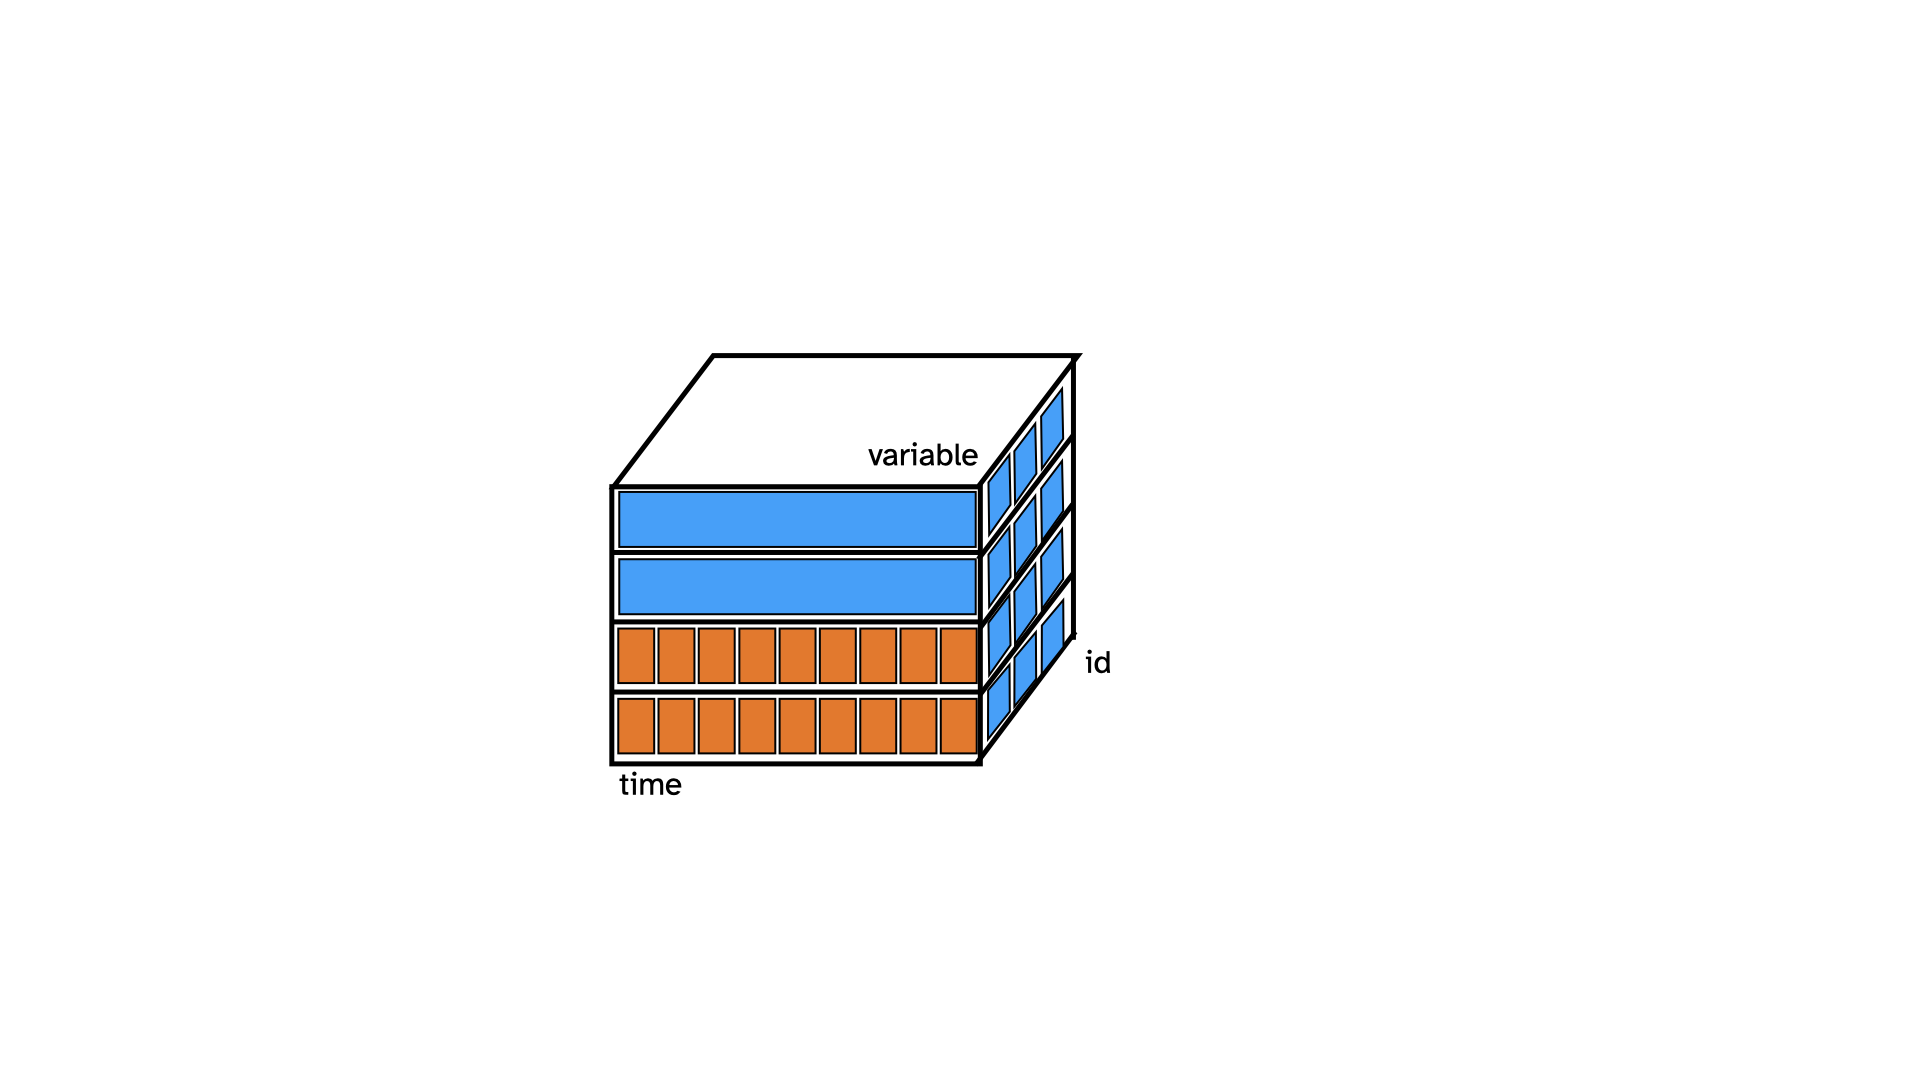
\includegraphics[width=1\linewidth]{../figures/diagram-keynotes/diagram-keynotes.007} 

}

\caption[An illustration of the conceptual spatio-temporal cube with different slicing on time, site, and variable]{An illustration of the conceptual spatio-temporal cube with different slicing on time, site, and variable. For each axis, the slicing can be on a single value or a set of values.}\label{fig:cube-def}
\end{figure}
\end{CodeChunk}

\hypertarget{cubble}{%
\section{The cubble package}\label{cubble}}

A \code{cubble} object is an S3 class \citep{advr} built on the \code{tibble} class, specifically to organise spatio-temporal data. The \code{cubble} class uses an attribute ``form'', to arrange the spatial or temporal data components tidily. The form attribute can take a value of either ``nested'' or ``long''. The nested cubble is a subclass of rowwise tibble (\code{rowwise_df}). It arranges each spatial site in a row, and uses list columns to store the feature geometry and the temporal information. The long cubble is a subclass of grouped tibble (\code{grouped_df}), which expands the temporal information into the long form and stores the spatial information in a ``spatial'' attribute.

The main functions in the package are \code{as_cubble()}, \code{face_spatial()}, \code{face_temporal()}, and \code{unfold()}. The following sections explain their roles, why the new cubble structure is needed and how the package relates to existing packages for spatial and temporal data analysis.

The dataset \texttt{climate\_flat} is used to illustrate \pkg{cubble} functionality. This is a subset from National Oceanic and Atmospheric Administration (NOAA) Global Historical Climatology Network Daily (GHCND) data. It contains spatial variables, station ID, latitude, longitude, elevation, station name, World Meteorology Organisation ID, in additional to daily temporal information, maximum and minimum temperature values and precipitation records for year 2020. The first five rows of \texttt{climate\_flat} are shown below:

\begin{CodeChunk}
\begin{CodeOutput}
# A tibble: 1,830 x 10
  id         lat  long  elev name  wmo_id date        prcp  tmax  tmin
  <chr>    <dbl> <dbl> <dbl> <chr>  <dbl> <date>     <dbl> <dbl> <dbl>
1 ASN0000~ -31.9  116.  15.4 pert~  94610 2020-01-01     0  31.9  15.3
2 ASN0000~ -31.9  116.  15.4 pert~  94610 2020-01-02     0  24.9  16.4
3 ASN0000~ -31.9  116.  15.4 pert~  94610 2020-01-03     6  23.2  13  
4 ASN0000~ -31.9  116.  15.4 pert~  94610 2020-01-04     0  28.4  12.4
5 ASN0000~ -31.9  116.  15.4 pert~  94610 2020-01-05     0  35.3  11.6
# ... with 1,825 more rows
\end{CodeOutput}
\end{CodeChunk}

\hypertarget{create}{%
\subsection{Create a cubble}\label{create}}

\textcolor{magenta}{A cubble can be created from various common spatio-temporal data formats, including basic R objects like tibble, tsibble, sf}. Section \ref{covid} describes converting multiple tables into a cubble object and Section \ref{netcdf} illustrates how to convert a netCDF object.

The function \code{as_cubble()} is used to create a cubble with three arguments: \code{key} as the spatial identifier; \code{index} as the temporal identifier; and a vector of \code{coords} in the order (longitude, latitude). The arguments \code{key} and \code{index} follow the wording in \pkg{tsibble} to describe the temporal order and multiple series while \code{coords} specifies the spatial location of each site. The code below creates a cubble out of \code{climate_flat} (a single tibble) with \code{id} as the key, \code{date} as the index, and \code{c(long, lat)} as the coordinates:

\begin{CodeChunk}
\begin{CodeInput}
R> cubble_nested <- climate_flat |>
+   as_cubble(key = id, index = date, coords = c(long, lat))
R> cubble_nested
\end{CodeInput}
\begin{CodeOutput}
# cubble:   id [5]: nested form
# bbox:     [115.97, -32.94, 133.55, -12.42]
# temporal: date [date], prcp [dbl], tmax [dbl], tmin [dbl]
  id            lat  long  elev name           wmo_id ts      
  <chr>       <dbl> <dbl> <dbl> <chr>           <dbl> <list>  
1 ASN00009021 -31.9  116.  15.4 perth airport   94610 <tibble>
2 ASN00010311 -31.9  117. 179   york            94623 <tibble>
3 ASN00010614 -32.9  117. 338   narrogin        94627 <tibble>
4 ASN00014015 -12.4  131.  30.4 darwin airport  94120 <tibble>
5 ASN00015131 -17.6  134. 220   elliott         94236 <tibble>
\end{CodeOutput}
\end{CodeChunk}

Printing a cubble provides some information about the data. \code{id} is the variable name to identify each location and there are five unique locations. The bounding box is \code{[115.97, -32.94, 133.55, -12.42]} and provides information about the coordinates in the data set. The third row shows the name and type of all variables nested in the \code{ts} column. In this example, it includes \code{date [date], prcp [dbl], tmax [dbl], tmin [dbl]}.

A cubble object is a subclass of the \code{rowwise_df} class where each row forms a group. All the temporal variables are nested in a list column, hence it is also called the nested cubble. The rowwise structure makes it simpler to operate on the list using the \code{mutate()} syntax, which is simpler than the \code{purr::map()} when working with a list column. For example, calculating the number of rainy days can be done by:

\begin{CodeChunk}
\begin{CodeInput}
R> cubble_nested |>
+   mutate(rain_day = sum(ts$prcp != 0))
\end{CodeInput}
\begin{CodeOutput}
# cubble:   id [5]: nested form
# bbox:     [115.97, -32.94, 133.55, -12.42]
# temporal: date [date], prcp [dbl], tmax [dbl], tmin [dbl]
  id            lat  long  elev name          wmo_id ts       rain_day
  <chr>       <dbl> <dbl> <dbl> <chr>          <dbl> <list>      <int>
1 ASN00009021 -31.9  116.  15.4 perth airport  94610 <tibble>      104
2 ASN00010311 -31.9  117. 179   york           94623 <tibble>       89
3 ASN00010614 -32.9  117. 338   narrogin       94627 <tibble>       90
4 ASN00014015 -12.4  131.  30.4 darwin airpo~  94120 <tibble>      106
5 ASN00015131 -17.6  134. 220   elliott        94236 <tibble>       63
\end{CodeOutput}
\end{CodeChunk}

\hypertarget{change-focus-by-facing-the-time-variables}{%
\subsection{Change focus by facing the time-variables}\label{change-focus-by-facing-the-time-variables}}

The nested form can be used for those operations where the output is only indexed by the spatial identifier (\code{key}), but becomes inadequate when outputs need both a spatial and a temporal identifier (\code{key} and \code{index}). The \pkg{cubble} class also provides a long form, which expands the \code{ts} column and temporarily ``hides'' the spatial variables. The function \code{face_temporal()} is used to switch from the nested cubble into the long one. The first row in Figure \ref{fig:face} illustrates this operation where the focus of the cube now changes from the site-variable face to the time-variable face. This code switches the cubble just created into its long form:

\begin{CodeChunk}
\begin{CodeInput}
R> cubble_long <- cubble_nested |> face_temporal()
R> cubble_long
\end{CodeInput}
\begin{CodeOutput}
# cubble:  date, id [5]: long form
# bbox:    [115.97, -32.94, 133.55, -12.42]
# spatial: lat [dbl], long [dbl], elev [dbl], name [chr], wmo_id
#   [dbl]
  id          date        prcp  tmax  tmin
  <chr>       <date>     <dbl> <dbl> <dbl>
1 ASN00009021 2020-01-01     0  31.9  15.3
2 ASN00009021 2020-01-02     0  24.9  16.4
3 ASN00009021 2020-01-03     6  23.2  13  
4 ASN00009021 2020-01-04     0  28.4  12.4
5 ASN00009021 2020-01-05     0  35.3  11.6
# ... with 1,825 more rows
\end{CodeOutput}
\end{CodeChunk}

The first line in the printed cubble now shows it in the long form and the third line has been changed to display the name and type of spatial variables: \code{lat [dbl], long [dbl], elev [dbl], name [chr], wmo_id [dbl]}. Unlike the nested form, the long cubble is built from a \code{grouped_df} class where all the observations from the same site form a group.

\begin{CodeChunk}
\begin{figure}

{\centering 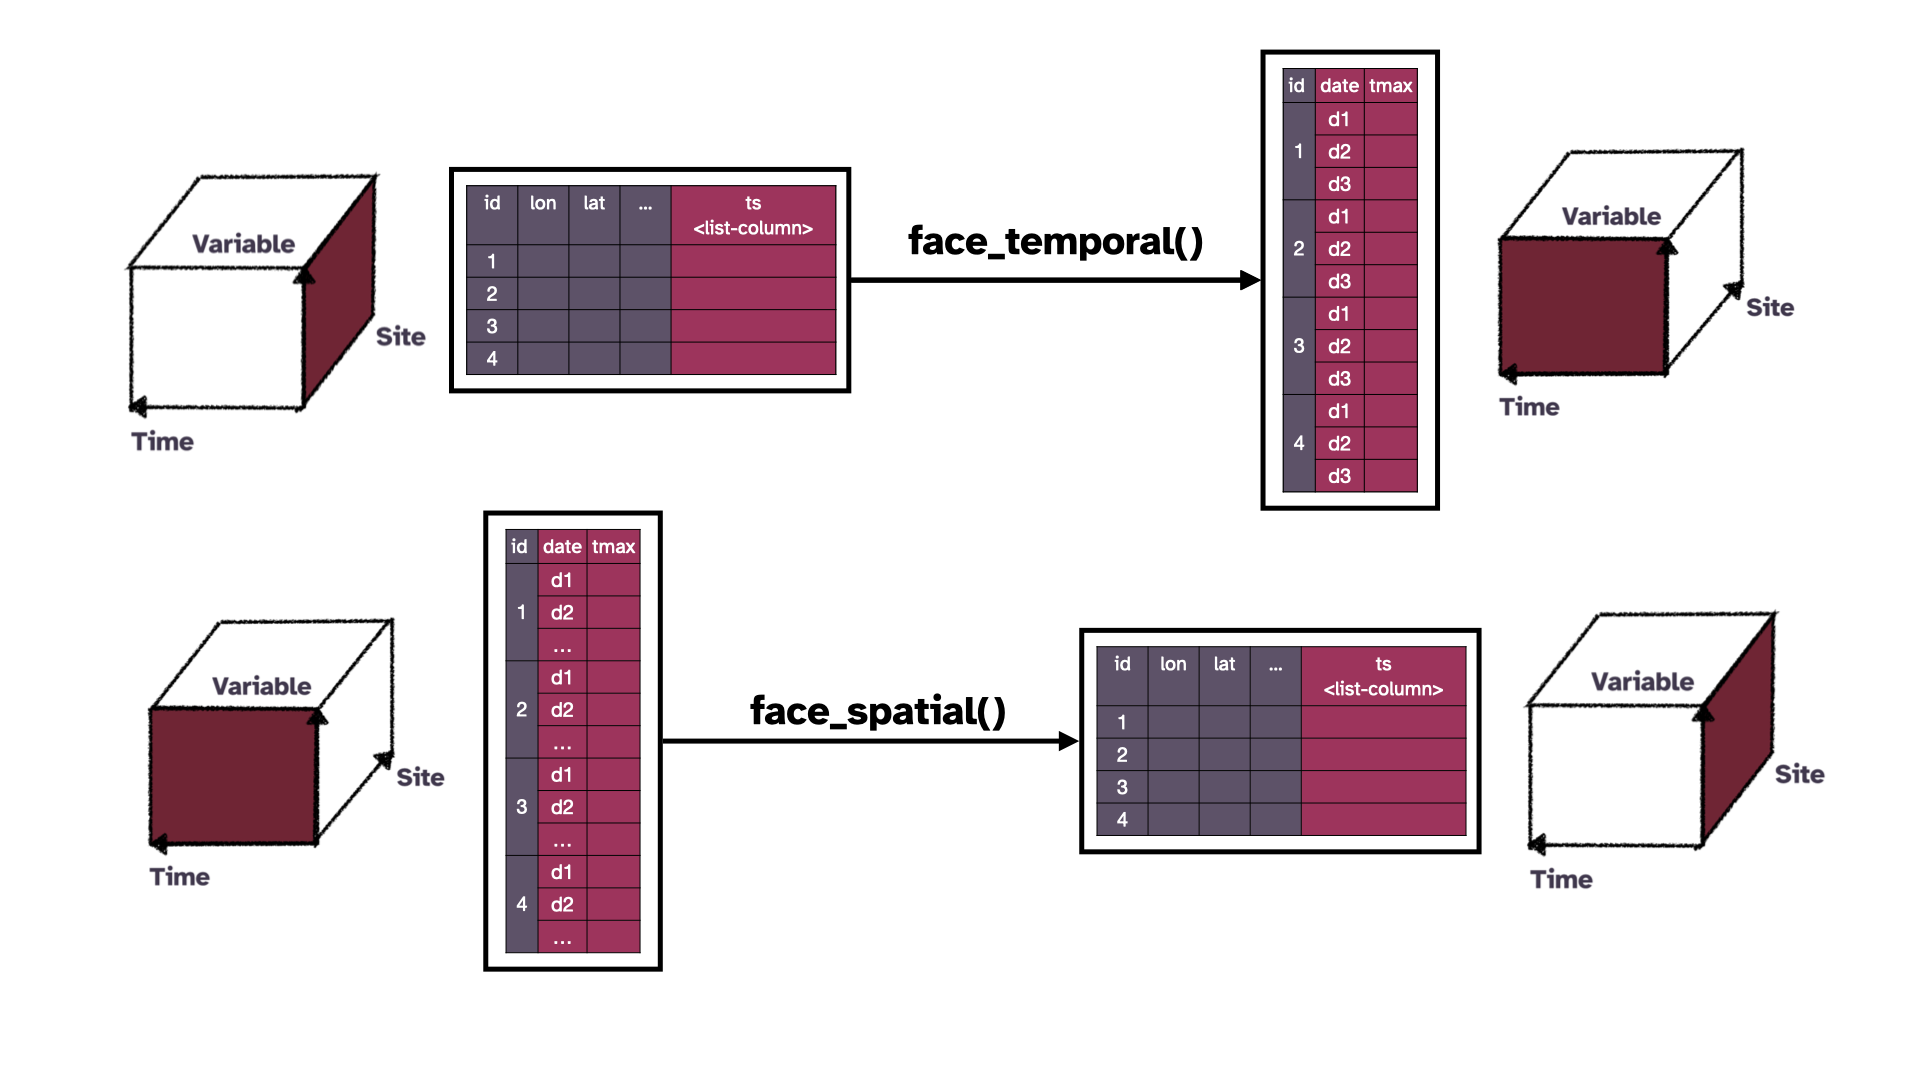
\includegraphics[width=1\linewidth]{../figures/diagram-keynotes/diagram-keynotes.008} 

}

\caption{An illustration of function \code{face\_temporal} and \code{face\_spatial} in cubble. In the first row, \code{face\_temporal} switches a cubble from the nested form into the long form and the focus has switched from the spatial aspect (the side face) to the temporal aspect (the front face). In the second row, \code{face\_spatial} switches a cubble back to the nested form from the long form and shifts focus back to the spatial aspect.}\label{fig:face}
\end{figure}
\end{CodeChunk}

\hypertarget{change-focus-back-to-the-site-variable-face}{%
\subsection{Change focus back to the site-variable face}\label{change-focus-back-to-the-site-variable-face}}

Wrangling spatio-temporal data can be seen as an iterative process in the spatial and temporal dimensions. Switching the focus back to the site-variable face can be accomplished by the function \code{face_spatial()}, which is the inverse of \code{face_temporal()}. The second row of Figure \ref{fig:face} illustrates the function, which is used as follows:

\begin{CodeChunk}
\begin{CodeInput}
R> cubble_back <- cubble_long |> face_spatial()
R> cubble_back
\end{CodeInput}
\begin{CodeOutput}
# cubble:   id [5]: nested form
# bbox:     [115.97, -32.94, 133.55, -12.42]
# temporal: date [date], prcp [dbl], tmax [dbl], tmin [dbl]
  id            lat  long  elev name           wmo_id ts      
  <chr>       <dbl> <dbl> <dbl> <chr>           <dbl> <list>  
1 ASN00009021 -31.9  116.  15.4 perth airport   94610 <tibble>
2 ASN00010311 -31.9  117. 179   york            94623 <tibble>
3 ASN00010614 -32.9  117. 338   narrogin        94627 <tibble>
4 ASN00014015 -12.4  131.  30.4 darwin airport  94120 <tibble>
5 ASN00015131 -17.6  134. 220   elliott         94236 <tibble>
\end{CodeOutput}
\begin{CodeInput}
R> identical(cubble_nested, cubble_back)
\end{CodeInput}
\begin{CodeOutput}
[1] TRUE
\end{CodeOutput}
\end{CodeChunk}

\hypertarget{unfold}{%
\subsection{Unfold spatial variables into the long cubble}\label{unfold}}

Sometimes, analysts may need to apply some variable transformation that involves both the spatial and temporal variables. An example of this is the transformation of temporal variables into the spatial dimension in glyph maps \citep{Wickham2012-yr}. (How to make glyph maps will be explained in Section \ref{st_transformation}, and are illustrated in the second example.) This type of operation can be seen as flattening, or \emph{unfolding}, the cube into a 2D data frame. Here the function \code{unfold()} moves the spatial variables \code{long} and \code{lat} into the long cubble:

\begin{CodeChunk}
\begin{CodeInput}
R> cubble_unfold <- cubble_long |> unfold(long, lat)
R> cubble_unfold
\end{CodeInput}
\begin{CodeOutput}
# cubble:  date, id [5]: long form
# bbox:    [115.97, -32.94, 133.55, -12.42]
# spatial: lat [dbl], long [dbl], elev [dbl], name [chr], wmo_id
#   [dbl]
  id          date        prcp  tmax  tmin  long   lat
  <chr>       <date>     <dbl> <dbl> <dbl> <dbl> <dbl>
1 ASN00009021 2020-01-01     0  31.9  15.3  116. -31.9
2 ASN00009021 2020-01-02     0  24.9  16.4  116. -31.9
3 ASN00009021 2020-01-03     6  23.2  13    116. -31.9
4 ASN00009021 2020-01-04     0  28.4  12.4  116. -31.9
5 ASN00009021 2020-01-05     0  35.3  11.6  116. -31.9
# ... with 1,825 more rows
\end{CodeOutput}
\end{CodeChunk}

This function should generally be used in the last step of the analysis since it is a temporary operation, meaning that these added spatial variables will disappear, if switched to the nested form and then switched back:

\begin{CodeChunk}
\begin{CodeInput}
R> cubble_unfold |> face_spatial() |> face_temporal()
\end{CodeInput}
\begin{CodeOutput}
# cubble:  date, id [5]: long form
# bbox:    [115.97, -32.94, 133.55, -12.42]
# spatial: lat [dbl], long [dbl], elev [dbl], name [chr], wmo_id
#   [dbl]
  id          date        prcp  tmax  tmin  long   lat
  <chr>       <date>     <dbl> <dbl> <dbl> <dbl> <dbl>
1 ASN00009021 2020-01-01     0  31.9  15.3  116. -31.9
2 ASN00009021 2020-01-02     0  24.9  16.4  116. -31.9
3 ASN00009021 2020-01-03     6  23.2  13    116. -31.9
4 ASN00009021 2020-01-04     0  28.4  12.4  116. -31.9
5 ASN00009021 2020-01-05     0  35.3  11.6  116. -31.9
# ... with 1,825 more rows
\end{CodeOutput}
\end{CodeChunk}

\hypertarget{tidyverse}{%
\subsection{Why not just use the existing tidyverse functions}\label{tidyverse}}

Some readers may question why a new data structure is needed rather than directly creating a list-column on the combined data using \code{dplyr::nest_by()}. The reason is that cubble is specifically designed to utilize the spatio-temporal structure when arranging observations in a single object. Moreover, it enables easy pivoting between purely spatial, purely temporal, or unfolded into a combined form.

\hypertarget{compact}{%
\subsection{Compatibility with existing packages}\label{compact}}

The \code{cubble} package leverages tools available in existing packages used for spatial and temporal analysis, specifically, \code{dplyr}, \code{tsibble}, \code{sf} (\code{s2}), and \code{netcdf4}, as explained here.

\hypertarget{dplyr}{%
\subsubsection{dplyr}\label{dplyr}}

The \code{dplyr} package has many tools for wrangling tidy data, many of which are useful in the spatio-temporal analysis. The \code{cubble} package provides \code{methods} that support the use of the following \code{dplyr} operations on both the nested and long forms: \texttt{mutate}, \texttt{filter}, \texttt{summarise}, \texttt{select}, \texttt{arrange}, \texttt{rename}, \texttt{left\_join}, and the slice family (\texttt{slice\_*}).

\hypertarget{tsibble}{%
\subsubsection{tsibble}\label{tsibble}}

A \code{tsibble} is a \code{tibble} where the \code{index} and \code{key} components are used to store temporal and strata information, that makes working with temporal data cognitively efficient. A \code{cubble} can use a \code{tsibble} for storing the temporal information, and effectively utilize the specialist time series operations in the \code{tsibble} package. It is easy to cast an existing \code{tsibble} into a \code{cubble} simply by supplying the \code{coords}:

\begin{CodeChunk}
\begin{CodeInput}
R> climate_flat_ts <- climate_flat |> 
+   tsibble::as_tsibble(key = id, index = date)
R> climate_flat_cb <-  climate_flat_ts |> 
+   cubble::as_cubble(coords = c(long, lat))
R> climate_flat_cb
\end{CodeInput}
\begin{CodeOutput}
# cubble:   id [5]: nested form
# bbox:     [115.97, -32.94, 133.55, -12.42]
# temporal: date [date], prcp [dbl], tmax [dbl], tmin [dbl]
  id            lat  long  elev name           wmo_id ts      
  <chr>       <dbl> <dbl> <dbl> <chr>           <dbl> <list>  
1 ASN00009021 -31.9  116.  15.4 perth airport   94610 <tbl_ts>
2 ASN00010311 -31.9  117. 179   york            94623 <tbl_ts>
3 ASN00010614 -32.9  117. 338   narrogin        94627 <tbl_ts>
4 ASN00014015 -12.4  131.  30.4 darwin airport  94120 <tbl_ts>
5 ASN00015131 -17.6  134. 220   elliott         94236 <tbl_ts>
\end{CodeOutput}
\end{CodeChunk}

When a nested cubble is created, each element in the list-column \code{ts} is a \code{tsibble} class (labelled \code{tbl_ts}) and operations available to the \code{tsibble} class are still valid on this element. For example, the code below calculates two time series features (mean and variance) of maximum temperature, utilizing the tsibble structure in the cubble:

\begin{CodeChunk}
\begin{CodeInput}
R> # add station-based features in the nested form.
R> climate_flat_cb |> 
+   mutate(
+     fabletools::features(
+       ts, tmax, list(tmax_mean = mean, tmax_var = var)
+       )
+   )
\end{CodeInput}
\begin{CodeOutput}
# cubble:   id [5]: nested form
# bbox:     [115.97, -32.94, 133.55, -12.42]
# temporal: date [date], prcp [dbl], tmax [dbl], tmin [dbl]
  id          lat  long  elev name  wmo_id ts       tmax_mean tmax_var
  <chr>     <dbl> <dbl> <dbl> <chr>  <dbl> <list>       <dbl>    <dbl>
1 ASN00009~ -31.9  116.  15.4 pert~  94610 <tbl_ts>      25.7    38.6 
2 ASN00010~ -31.9  117. 179   york   94623 <tbl_ts>      26.2    51.1 
3 ASN00010~ -32.9  117. 338   narr~  94627 <tbl_ts>      23.7    45.4 
4 ASN00014~ -12.4  131.  30.4 darw~  94120 <tbl_ts>      33.1     3.02
5 ASN00015~ -17.6  134. 220   elli~  94236 <tbl_ts>      34.6    24.7 
\end{CodeOutput}
\end{CodeChunk}

\hypertarget{sf-and-s2}{%
\subsubsection{sf and s2}\label{sf-and-s2}}

The \code{sf} is a spatial data object, containing a feature geometry list-column (\code{sfc}) in the form of various geometry types (\code{POINT}, \code{LINESTRING}, \code{POLYGON}, \code{MULTIPOLYGON}). The \code{sf} package provides functions that operate efficiently on this spatial information. A cubble can store the spatial information as an \code{sf} object. Methods for the \code{sfc} class can be applied in the nested form of the cubble object. An illustration is in Section \ref{covid}. A spatial data object with an \code{s2} vector can also be used to store the spatial information in a \code{cubble}.

\hypertarget{netcdf}{%
\subsubsection{netCDF}\label{netcdf}}

NetCDF data is another format commonly used for storing spatio-temporal data. It has two main components: \emph{dimension} for defining the spatio-temporal grid (longitude, latitude, and time) and \emph{variable} that populates the defined grid. Attributes can be associated with dimensions or variables. Because there can be many different styles of representing this information there is a metadata convention \citep{hassell_data_2017} to standardise the format of the attributes. A few packages in R exist for manipulating NetCDF data and these include a high-level R interface: \pkg{ncdf4} \citep{ncdf4}, a low-level interface that calls a C-interface: \pkg{RNetCDF} \citep{rnetcdf}, and a tidyverse implementation: \pkg{tidync} \citep{tidync}.

Cubble provides an \code{as_cubble()} method to coerce the \code{ncdf4} class from the \pkg{ncdf4} package into a \code{cubble}. It maps each combination of longitude and latitude into an \code{id} as the \code{key}:

\begin{CodeChunk}
\begin{CodeInput}
R> # read in the .nc file as a ncdf4 class
R> raw <- ncdf4::nc_open(here::here("data/era5-pressure.nc"))
R> 
R> # convert the variable q and z in the ncdf4 into a cubble
R> dt <- as_cubble(raw, vars = c("q", "z"))
\end{CodeInput}
\end{CodeChunk}

NetCDF data can be quite large, and it is sometimes best to subset the data when converting to a cubble. We would recommend reducing to about 300 \(\times\) 300 grid points for three daily variables in one year. A 300 by 300 spatial grid can be a bounding box of {[}100, -80, 180, 0{]} at 0.25 degree resolution or a global bounding box {[}-180, -90, 180, -90{]} at 1 degree resolution.
The size of spatial grid can be reduced if longer time periods or more variables are needed, through \code{long_range} and \code{lat_range}:

\begin{CodeChunk}
\begin{CodeInput}
R> # Assume my_ncdf has a bounding box of [-180, -90, 180, -90]
R> # at 0.25 degree resolution and subset it to have
R> # 1 degree resolution:
R> dt <- as_cubble(my_ncdf, vars = c("q", "z"),
+                 long_range = seq(-180, 180, 1),
+                 lat_range = seq(-90, 90, 1))
\end{CodeInput}
\end{CodeChunk}

\hypertarget{others}{%
\section{Other features and considerations}\label{others}}

\hypertarget{hierarchical-structure}{%
\subsection{Hierarchical structure}\label{hierarchical-structure}}

Spatial locations can have grouping structures either inherent to the data (e.g.~state within country) or obtained during the analysis (e.g.~cluster id). In this case, it can be useful to summarise variables at various levels of the hierarchy. The function \code{switch_key()} can be used to change the grouping level of spatial locations. The diagram in Figure \ref{fig:illu-hier} shows how this function can be used to switch the grouping from station ids to cluster ids. The result can also be stretched into long form. By specifying

\code{cluster_nested <- station_nested \%>\% switch_key(key = cluster)},

the cubble redefines the cubble key from the \code{id} column in \code{station_nested} to the \code{cluster} column in \code{cluster_nested}. All the spatial variables belonging to the \code{cluster} column are now nested into a \code{.val} column which allows for summarizing based on cluster.

\begin{CodeChunk}
\begin{figure}

{\centering 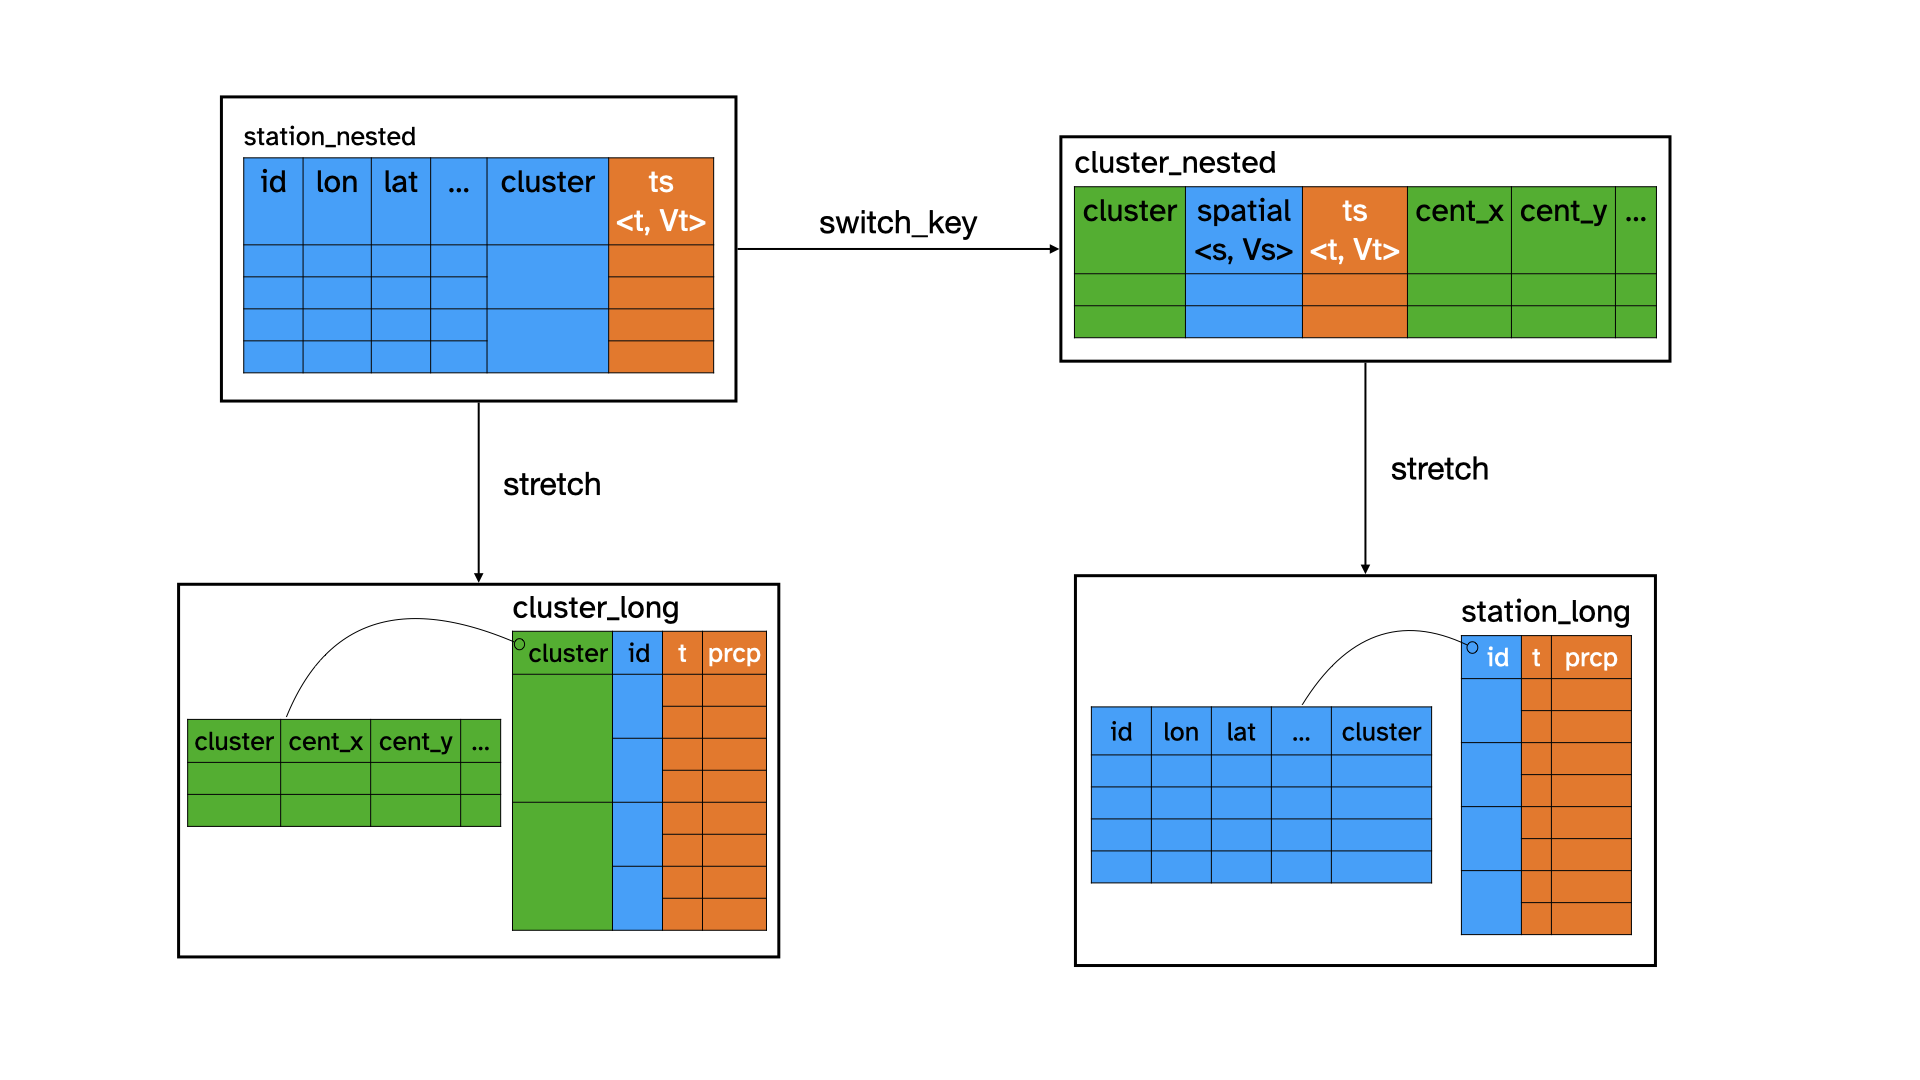
\includegraphics[width=1\linewidth,height=0.4\textheight]{../figures/diagram-keynotes/diagram-keynotes.003} 

}

\caption[Hierarchical spatial structure can be handled using \code{switch\_key()}, to create summaries based on any level]{Hierarchical spatial structure can be handled using \code{switch\_key()}, to create summaries based on any level. Here the switch is between the station id and a cluster id. Once the change is made the data can be stretched into the long form.}\label{fig:illu-hier}
\end{figure}
\end{CodeChunk}

\hypertarget{matching}{%
\subsection{Data fusion and matching}\label{matching}}

One task that may interest spatio-temporal analysts is combining data collected at nearby but not exactly the same sites, for example, weather station measured rainfall and river levels. This can be considered to be a matching problem \citep{stuart2010matching, mcintosh2018using} to pair similar time series from nearby locations, or even a data fusion exercise that merges data collected from different sources \citep{cocchi2019data}. The function \code{match_sites()} in \pkg{cubble} provides a simple algorithm for this task. The algorithm first matches spatially by computing the pairwise distance on latitude and longitude. Then it matches temporally by computing the number of matched peaks within a fixed length moving window. Figure \ref{fig:illu-matching} illustrates this temporal matching. In the two series, \code{A} and \code{a}, three peaks have been identified in each. An interval, of fixed length, is constructed for each peak in series \code{A}, while the peaks in series \code{a} are tested against whether they fall into any of the intervals. Here two out of three peaks match. Options for \code{match_sites()} are:

\begin{CodeChunk}
\begin{figure}

{\centering 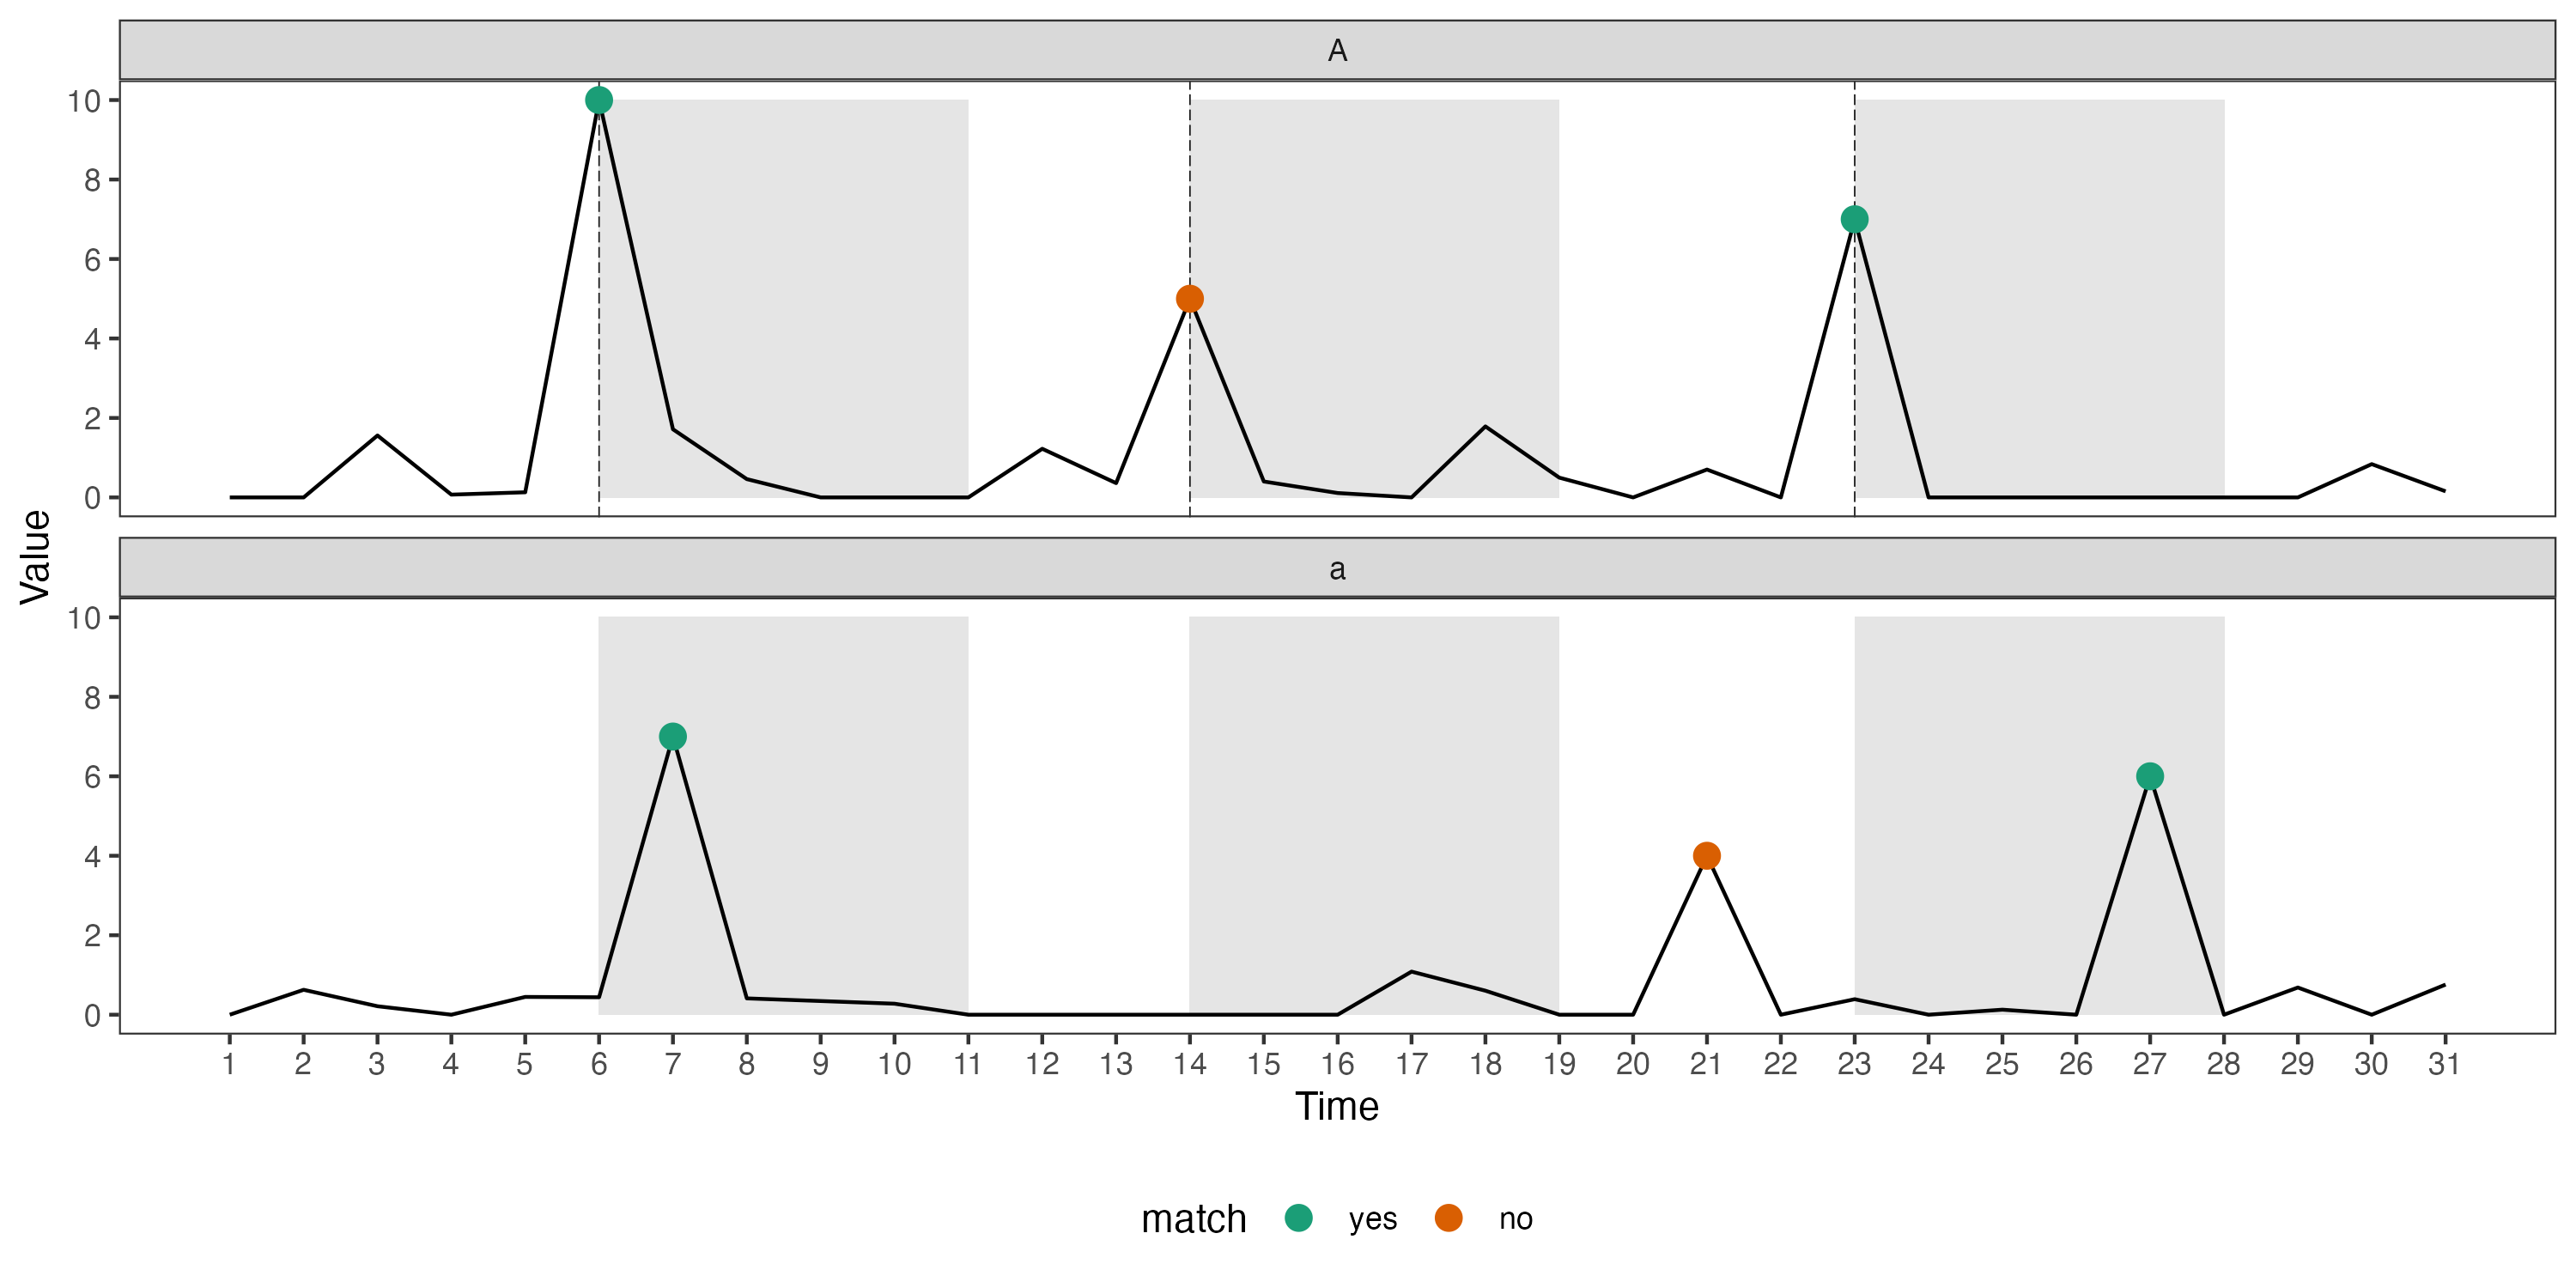
\includegraphics[width=1\linewidth]{../figures/illu-matching} 

}

\caption{An illustration of temporal matching in cubble. Three highest peaks are identified in each series and intervals are constructed on series \code{A}. Two peaks in series \code{a} fall into the intervals and hence the two series are considered to have two matches.}\label{fig:illu-matching}
\end{figure}
\end{CodeChunk}

\begin{itemize}
\tightlist
\item
  \code{spatial_n_keep}: the number of spatial match for each site to keep
\item
  \code{spatial_dist_max}: the maximum distance allowed for a matched pair
\item
  \code{temporal_n_highest}: the number of peaks used - 3 in the example above
\item
  \code{temporal_window}: the length of the interval - 5 in the example above
\item
  \code{temporal_min_match}: the minimum number of matched peaks for a valid matched pair
\end{itemize}

\hypertarget{interactive-graphics}{%
\subsection{Interactive graphics}\label{interactive-graphics}}

The cubble workflow fits works well with an interactive graphics pipeline (e.g. \citet{buja1988elements}, \citet{buja1996interactive}, \citet{sutherland2000orca}, \citet{xie2014reactive}, \citet{cheng2016enabling}) that is available in R with the package crosstalk \citep{crosstalk}. Figure \ref{fig:illu-interactive} illustrates how linking can be achieved between a map and multiple time series using a cubble. The map (produced from the nested form) and time series (produced from the long form) are both shared crosstalk objects. When a user makes a selection on the map, the site is highlighted (left). This activates a row in the nested cubble object, which is then communicated to the long cubble -- all the observations with the same \code{id} (middle) will be selected. The long cubble will then highlight the corresponding series in the time series plot (right).

Linking is also available starting from the time series plot, by selecting points. This will be activate rows having the same \code{id} in the long cubble. The corresponding rows in the nested cubble are activated, and highlighted the map. (An illustration can be found in the appendix.) Note that this type of linking, both from the map or the time series, is what \citet{CS07} would call categorical variable linking, where station id is the categorical variable.

\begin{CodeChunk}
\begin{figure}

{\centering 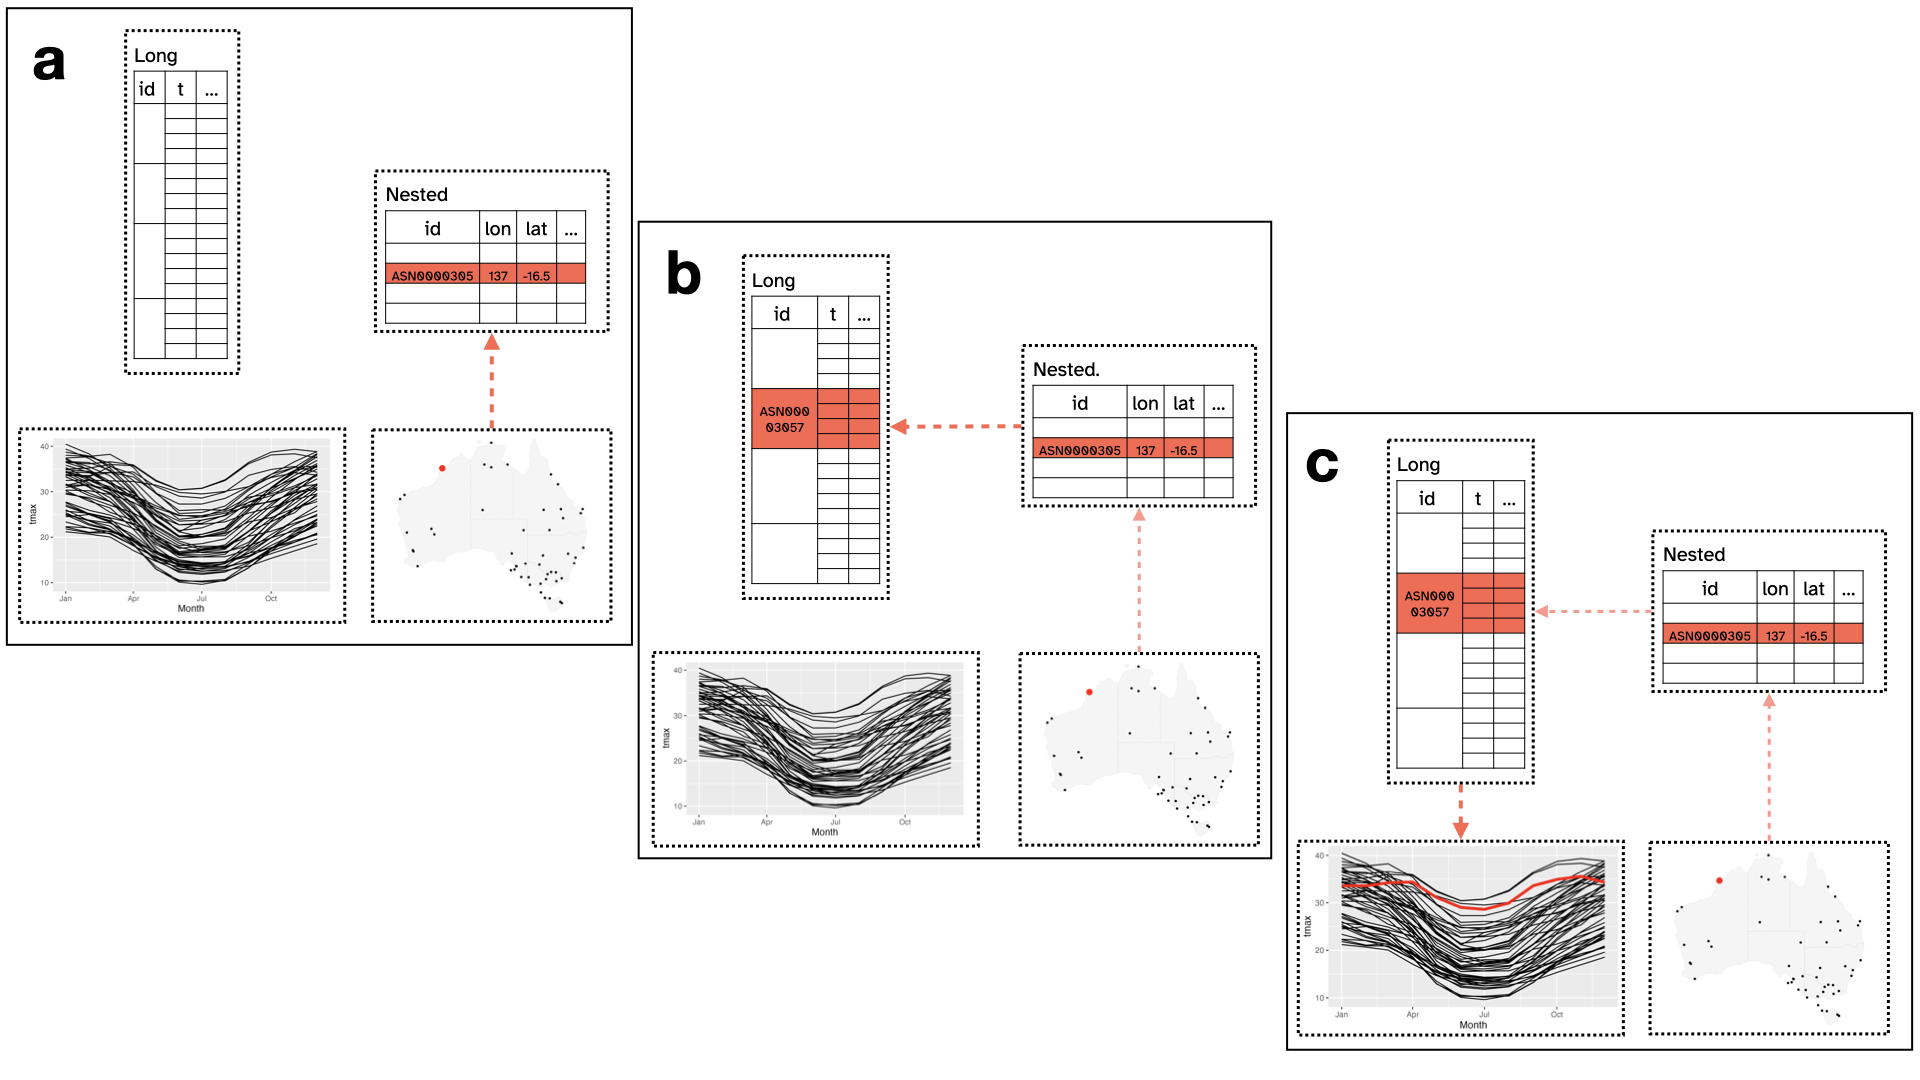
\includegraphics[width=1\linewidth,height=0.4\textheight]{../figures/diagram-keynotes/diagram-keynotes.004} 

}

\caption[An illustration of the data model under interactive graphics with cubble]{An illustration of the data model under interactive graphics with cubble. The line plot and the map is made separately with the long and nested cubble. When a station is selected on the map (left), the corresponding row in the nested cubble will be activated. This will link to all the rows with the same id in the long cubble (middle) and update the line plot (right).}\label{fig:illu-interactive}
\end{figure}
\end{CodeChunk}

\hypertarget{st_transformation}{%
\subsection{Spatio-temporal transformations}\label{st_transformation}}

Spatio-temporal data lends itself to a range of transformations. Glyph maps (Section \ref{unfold}) transform the measured variable and time coordinates into microplots at the spatial locations. Calendar plots \citep{wang2020calendar} deconstruct time to produce plots of variables in a calendar format. Summarising multiple variables is commonly done using projections, or linear combinations. Here we elaborate on the transformations made to produce a glyph map.

The \proglang{R} package \pkg{GGally} implements glyph maps through the \code{glyphs()} function. The function constructs a data frame with calculated position (\code{gx}, \code{gy}, \code{gid}) of each point on the time series using linear algebra (Equations 1 and 2 in \citet{Wickham2012-yr}). The data can then be piped into \code{ggplot} to create the glyph map as:

\begin{CodeChunk}
\begin{CodeInput}
R> library(ggplot2)
R> gly <- glyphs(data,
+               x_major = ..., x_minor = ...,
+               y_major = ..., y_minor = ..., ...)
R> 
R> ggplot(gly, aes(gx, gy, group = gid)) +
+   geom_path()
\end{CodeInput}
\end{CodeChunk}

A new implementation of the glyph map as a ggproto, \code{GeomGlyph}, has been made in the \pkg{cubble} package so that a glyph map can be created with \code{geom_glyph()}:

\begin{CodeChunk}
\begin{CodeInput}
R> ggplot(data = data) +
+   geom_glyph(aes(x_major = ..., x_minor = ...,
+                  y_major = ..., y_minor = ...))
\end{CodeInput}
\end{CodeChunk}

An example using a glyph map is shown in Section \ref{precip}.

Some useful controls over the glyph map are also available in the \code{geom_glyph()} implementation. Polar coordinate glyph maps are specified using \code{polar = TRUE}, and parameters \code{width} and \code{height} can be specified in either absolute or relative value. Global and local scale is specified with \code{global_rescale}, which defaults to \code{TRUE}. Reference boxes and lines can be added with separate \code{geom_glyph_box()} and \code{geom_glyph_line()} lines.

\hypertarget{examples}{%
\section{Examples}\label{examples}}

\hypertarget{covid}{%
\subsection{Victoria covid data}\label{covid}}

The Victoria State Government in Australia provides daily COVID information about the source and local government area (LGA) of recorded cases. This data can be used to visualise COVID spread when combined with map information available from the Australian Bureau of Statistics. Here we will use the data to demonstrate how to match sites between these two tables with \pkg{cubble} in the case of a few mismatches. The first five rows these data sets are printed below:

\begin{CodeChunk}
\begin{CodeInput}
R> covid |> head(5)
\end{CodeInput}
\begin{CodeOutput}
# A tsibble: 5 x 5 [1D]
# Key:       lga [1]
# Groups:    lga, source [1]
  date       lga        source                            n roll_mean
  <date>     <chr>      <chr>                         <int>     <dbl>
1 2022-01-01 Alpine (S) Contact with a confirmed case     1        NA
2 2022-01-02 Alpine (S) Contact with a confirmed case     2        NA
3 2022-01-03 Alpine (S) Contact with a confirmed case     4        NA
4 2022-01-04 Alpine (S) Contact with a confirmed case     4        NA
5 2022-01-05 Alpine (S) Contact with a confirmed case     2        NA
\end{CodeOutput}
\begin{CodeInput}
R> lga |> head(5)
\end{CodeInput}
\begin{CodeOutput}
Simple feature collection with 5 features and 7 fields
Geometry type: MULTIPOLYGON
Dimension:     XY
Bounding box:  xmin: 142.3535 ymin: -38.67876 xmax: 147.3909 ymax: -36.39269
Geodetic CRS:  WGS 84
    lga_code_2018            lga state_code_2016 state_name_2016
132         20110     Alpine (S)               2        Victoria
133         20260    Ararat (RC)               2        Victoria
134         20570   Ballarat (C)               2        Victoria
135         20660    Banyule (C)               2        Victoria
136         20740 Bass Coast (S)               2        Victoria
    areasqkm_2018 cent_long  cent_lat                       geometry
132     4788.1568  146.9742 -36.85357 MULTIPOLYGON (((146.7258 -3...
133     4211.1171  142.8432 -37.47271 MULTIPOLYGON (((143.1807 -3...
134      739.0321  143.7815 -37.49286 MULTIPOLYGON (((143.6622 -3...
135       62.5402  145.0851 -37.73043 MULTIPOLYGON (((145.1357 -3...
136      865.8095  145.5581 -38.50730 MULTIPOLYGON (((145.5207 -3...
\end{CodeOutput}
\end{CodeChunk}

A \code{cubble} object can be created from separate spatial and temporal tables in a list, the other arguments (\code{key}, \code{index}, and \code{coords}) are described in section \ref{create}. The function \code{as_cubble()} will automatically try to match the sites in both tables and show a warning message in case of missing information (mismatch between the sites in the two tables).

\begin{CodeChunk}
\begin{CodeInput}
R> cb <- as_cubble(
+   list(spatial = lga, temporal = covid),
+   key = lga, index = date, coords = c(cent_long, cent_lat)
+   )
\end{CodeInput}
\begin{CodeOutput}
! Some sites in the temporal table don't have spatial information
\end{CodeOutput}
\begin{CodeOutput}
! Some sites in the spatial table don't have temporal information
\end{CodeOutput}
\begin{CodeOutput}
! Use argument `output = "unmatch"` to check on the unmatched key
\end{CodeOutput}
\begin{CodeOutput}
Joining, by = "lga"
\end{CodeOutput}
\end{CodeChunk}

In the output above we see that this is an issue here, and we proceed to use \code{output = "unmatch"} to check which locations are concerned. Note that \pkg{cubble} will attempt to pair the unmatched sites, these are shown separately from the ones that cannot be paired.

\begin{CodeChunk}
\begin{CodeInput}
R> pair <- as_cubble(
+   list(spatial = lga, temporal = covid),
+   key = lga, index = date, coords = c(cent_long, cent_lat),
+   output = "unmatch"
+   )
R> 
R> pair
\end{CodeInput}
\begin{CodeOutput}
$paired
# A tibble: 2 x 2
  spatial             temporal    
  <chr>               <chr>       
1 Kingston (C) (Vic.) Kingston (C)
2 Latrobe (C) (Vic.)  Latrobe (C) 

$others
$others$temporal
[1] "Interstate" "Overseas"   "Unknown"   

$others$spatial
[1] "No usual address (Vic.)"               
[2] "Migratory - Offshore - Shipping (Vic.)"
\end{CodeOutput}
\end{CodeChunk}

This information is helpful when cleaning up the data before creating the cubble again:

\begin{CodeChunk}
\begin{CodeInput}
R> lga <- lga %>%
+   mutate(lga = ifelse(lga == "Kingston (C) (Vic.)", "Kingston (C)", lga),
+          lga = ifelse(lga == "Latrobe (C) (Vic.)", "Latrobe (C)", lga)) %>%
+   filter(!lga %in% pair$others$spatial)
R> 
R> covid <- covid %>% filter(!lga %in% pair$others$temporal)
R> 
R> cb <- as_cubble(data = list(spatial = lga, temporal = covid),
+                 key = lga, index = date, coords = c(cent_long, cent_lat))
\end{CodeInput}
\end{CodeChunk}

\hypertarget{australian-historical-maximum-temperature}{%
\subsection{Australian historical maximum temperature}\label{australian-historical-maximum-temperature}}

The Global Historical Climatology Network (GHCN) provides daily climate measures from stations across the world. The \textbf{cubble} dataset \code{weatherdata::historical_tmax} extracts the maximum temperature for 204 Australian stations from the GHCN starting from year 1969 and provides information also on the latitude, longitude and elevation of each of the stations. This \textbf{cubble} data is already cast into a \code{cubble} data object, with \code{id} as the key, \code{date} as the index, and \code{c(longitude, latitude)} as the coordinates. The goal of this example is to compare the monthly average maximum temperature between two periods, 1971-1975 and 2016-2020, for stations in Victoria and New South Wales.

First of all, the stations across the two states need to be subsetted from the original data set \code{weatherdata::historical_tmax}. For that, the country and the station identifiers, stored within the 11 digits of the \code{id} variable entries, need to be retrieved. The country code is located in the first 5 digits (Australia is represented by ``ASN00'') while the next 6 digits encode the station information following the \href{http://www.bom.gov.au/climate/cdo/about/site-num.shtml}{Australian Bureau of Meteorology (BOM)} coding protocols. According to those, New South Wales stations correspond to entries in the range 46-75 and the Victorian stations are stored under 76-90. Filtering Victoria and New South Wales stations is a spatial operation and hence uses the \code{cubble} nested form:

\begin{CodeChunk}
\begin{CodeInput}
R> tmax <- weatherdata::historical_tmax |>
+   filter(between(stringr::str_sub(id, 7, 8), 46, 90))
\end{CodeInput}
\end{CodeChunk}

and extracting the time periods 1971-1975 and 2016-2020 is a time operation and therefore the nested cubble needs to be switched to the long cubble form by \code{stretch()}:

\begin{CodeChunk}
\begin{CodeInput}
R> tmax <- tmax |>
+   face_temporal() |>
+   filter(lubridate::year(date) %in% c(1971:1975, 2016:2020))
\end{CodeInput}
\end{CodeChunk}

A monthly maximum average temperature is then calculated for both periods where \code{cubble} easily allows to compute this time operation across all the stations:

\begin{CodeChunk}
\begin{CodeInput}
R> tmax <- tmax |>
+   group_by(month = lubridate::month(date),
+          group = as.factor(ifelse(lubridate::year(date) > 2015,
+                                   "2016 ~ 2020", "1971 ~ 1975"))) |>
+   summarise(tmax = mean(tmax, na.rm = TRUE))
\end{CodeInput}
\end{CodeChunk}

Observing the results of the operation above show that a few stations do not have records during the time period 1971-1975. Further investigation shows that while the first and last year of each series for those stations are recorded, the years in between are not. Hence, these stations are located and filtered out by examining whether the summarised time series has 24 months. Here, the long cubble needs to be switched to the nested form to carry out this spatial operation using \code{face_spatial()}:

\begin{CodeChunk}
\begin{CodeInput}
R> tmax <- tmax |> face_spatial() |> filter(nrow(ts) == 24)
\end{CodeInput}
\end{CodeChunk}

Lastly, to create a glyph map where the series of each station are overlayed on a map of Australia, both the major (\code{longitude}, \code{latitude}) and minor (\code{month}, \code{tmax}) coordinates defining the bounding box for the plot need to be on the same table. For that, spatial variables can be moved to the long form with \code{unfold()}:

\begin{CodeChunk}
\begin{CodeInput}
R> tmax <- tmax |> face_temporal() |> unfold(latitude, longitude)
\end{CodeInput}
\end{CodeChunk}

the variable storing the maximum monthly average temperatures \code{tmax} can then be supplied to \code{geom_glyph()} for the glyph map in Figure \ref{fig:basic-manip} with a station inset on the top left corner:

\begin{CodeChunk}
\begin{CodeInput}
R> nsw_vic <- ozmaps::abs_ste |>
+   filter(NAME %in% c("Victoria", "New South Wales"))
R> 
R> ggplot() +
+   geom_sf(data = nsw_vic,
+           fill = "transparent", color = "grey", linetype = "dotted") +
+   geom_glyph(data = tmax,
+              aes(x_major = longitude, x_minor = month,
+                  y_major = latitude, y_minor = tmax,
+                  group = interaction(id, group), color = group),
+              width = 1, height = 0.5) +
+   ...
\end{CodeInput}
\end{CodeChunk}

\begin{CodeChunk}
\begin{figure}

{\centering 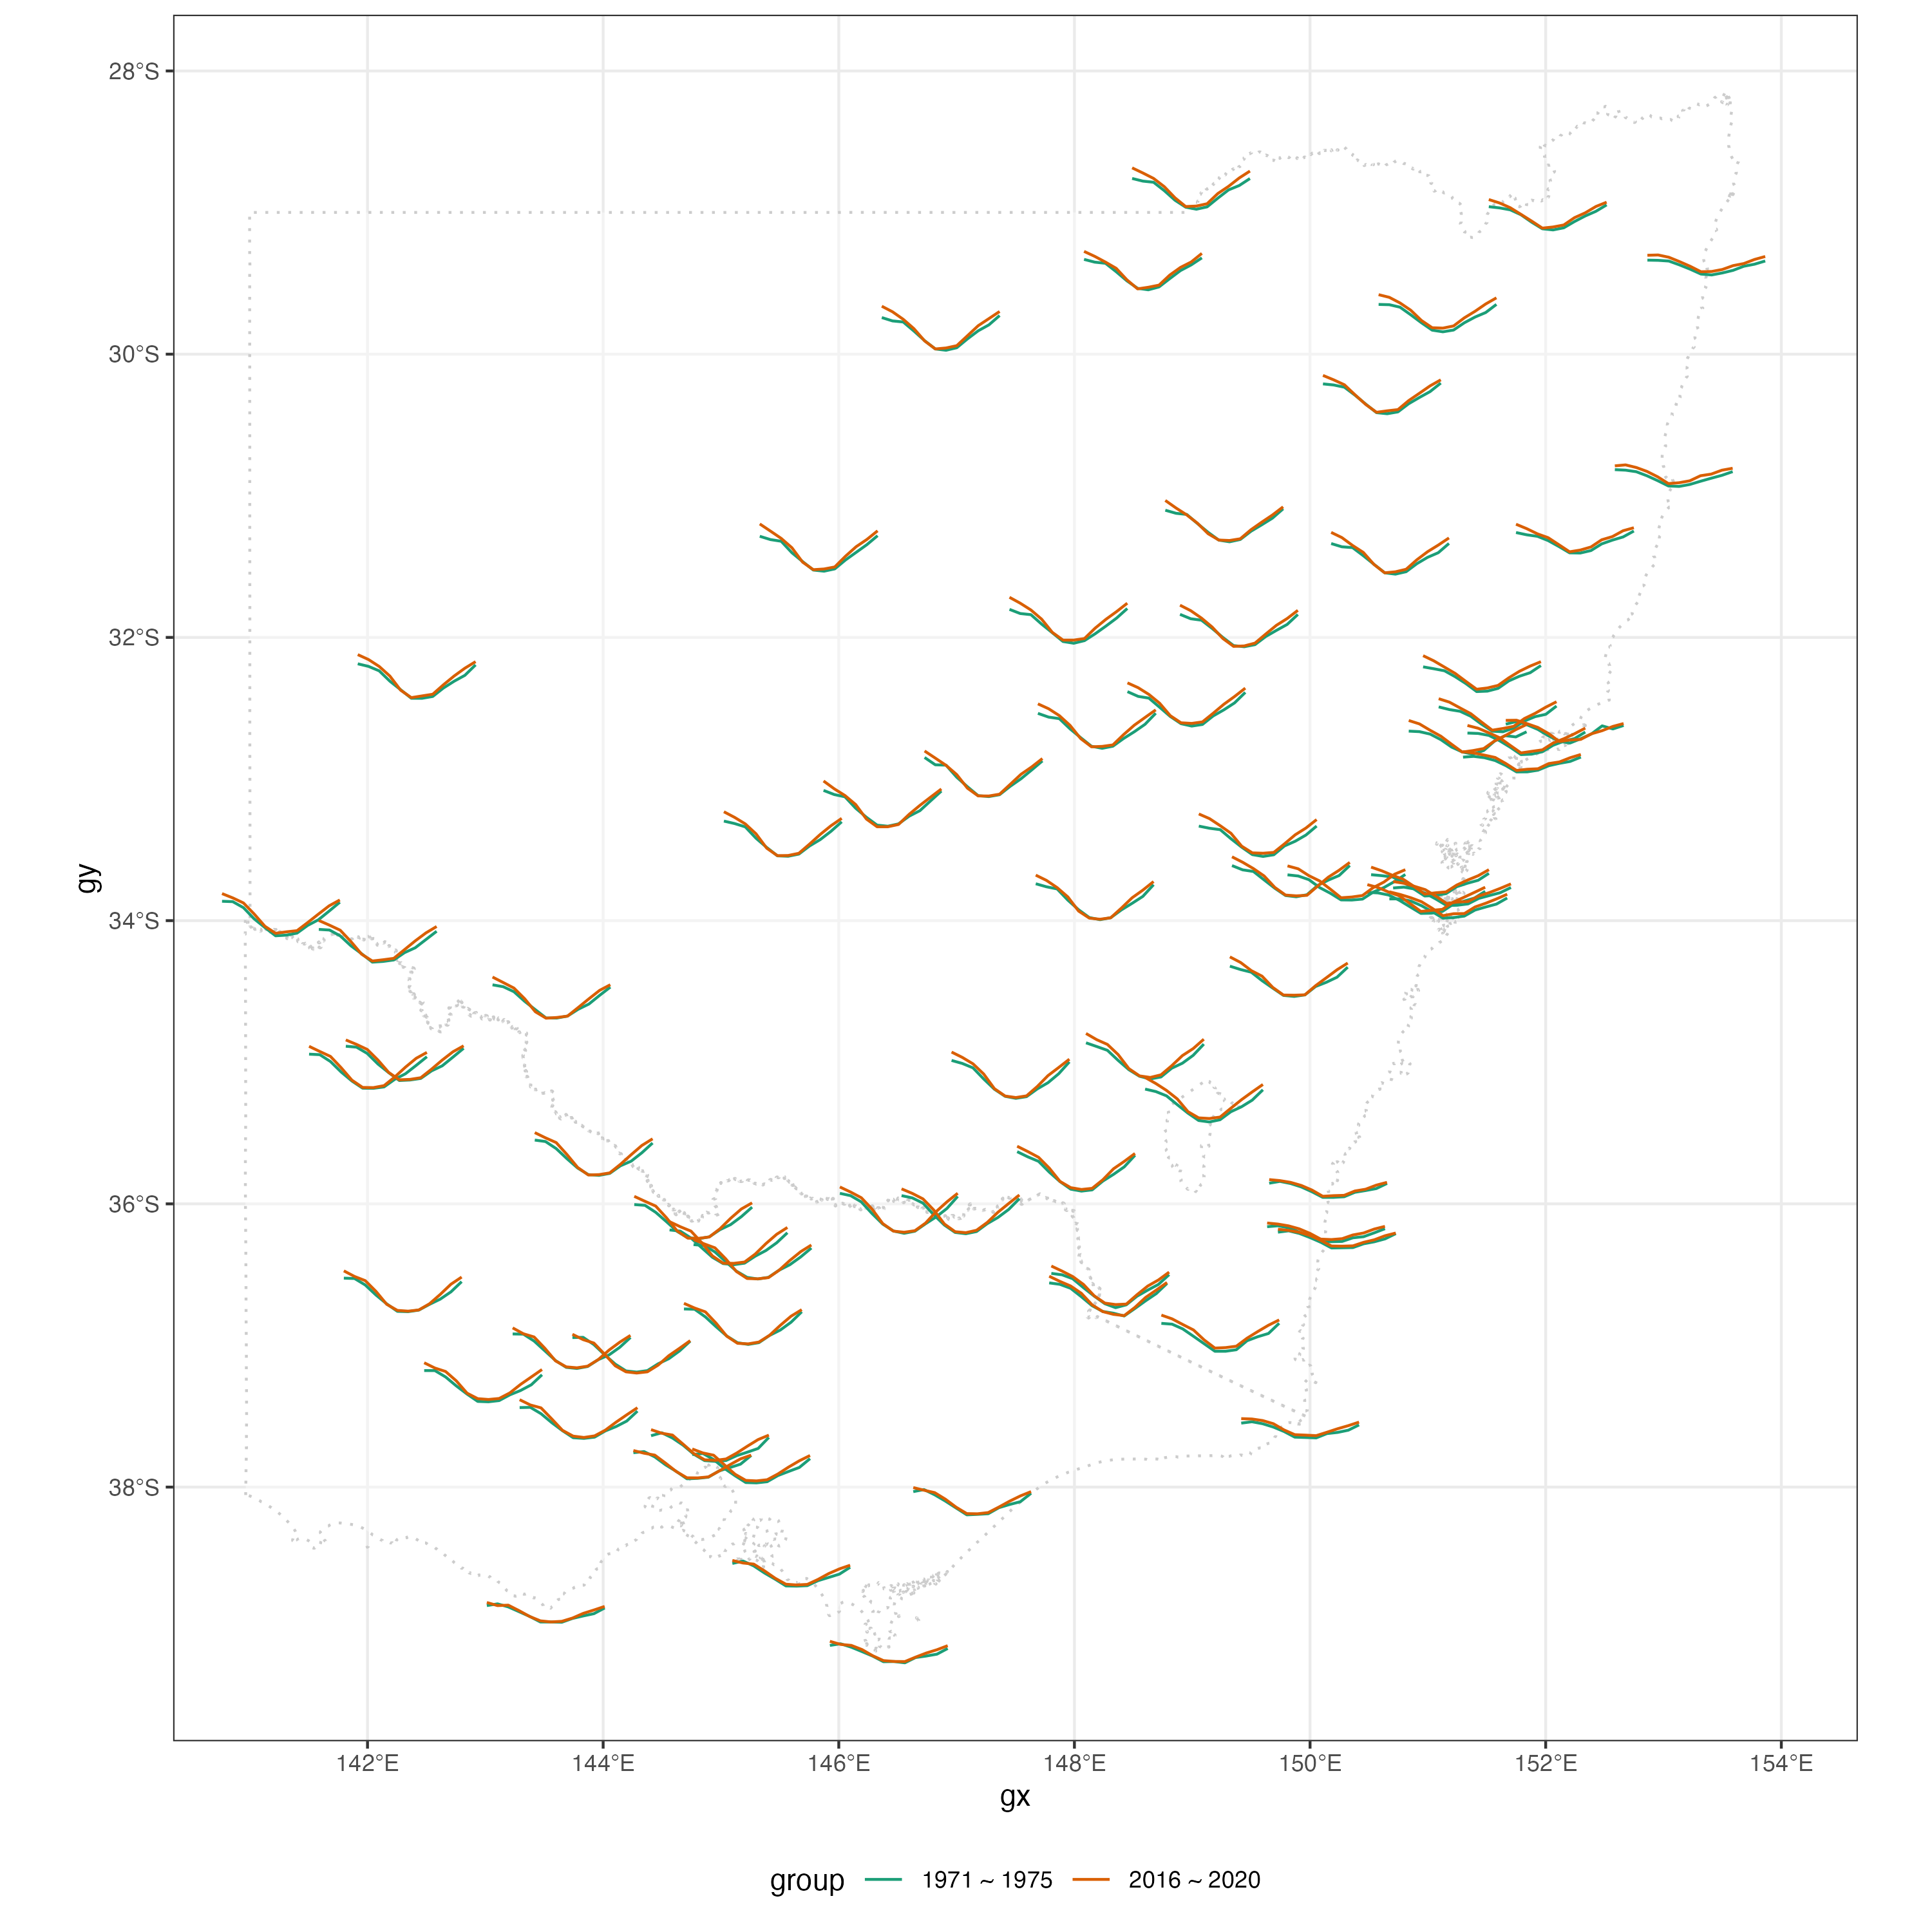
\includegraphics[width=0.9\linewidth]{../figures/basic-manip} 

}

\caption[A glyph map of the average maximum temperature by month for parts of Victoria and New South Wales weather stations in Australia for two five year periods (1971-1975, 2016-2020)]{A glyph map of the average maximum temperature by month for parts of Victoria and New South Wales weather stations in Australia for two five year periods (1971-1975, 2016-2020). An inset (top left) showing detail is the station Cobar (highlighted by black rectangle). The mothly trend is similar at all locations (low in the winter, high in the summer), and small increased temperatures, particularly in late summer can be seen at most stations.}\label{fig:basic-manip}
\end{figure}
\end{CodeChunk}

\hypertarget{precip}{%
\subsection{Australian precipitation pattern in 2020}\label{precip}}

In the previous example, some overlapping of the glyphs occurred for a few nearby stations such as the pairs (151E, 34S) and (152E, 33S). This is a problem when mapping more stations at the national level. Aggregation can be helpful in grouping series into clusters before visualising the clusters with a glyph map. This new example shows how to organise data at both levels with \code{switch_key()}.

\code{weatherdata::climate_full}, also extracted from the GHCN, records daily precipitation and maximum/minimum temperature for 640 stations in Australia from 2016 to 2020. A simple \(k\)-means algorithm based on the distance matrix between stations is used to create 20 clusters. The dataset \code{station_nested} is a nested cubble with a cluster column indicating the group to which each station belongs. More advanced clustering algorithms can be used as well, as long as they provide a mapping from each station to a cluster.

\begin{CodeChunk}
\begin{CodeInput}
R> station_nested <- weatherdata::climate_full |> mutate(cluster = ...)
\end{CodeInput}
\end{CodeChunk}

To create a group-level cubble, use \code{switch_key()} with the new key variable, \code{cluster}:

\begin{CodeChunk}
\begin{CodeInput}
R> cluster_nested <- station_nested |> switch_key(cluster)
\end{CodeInput}
\end{CodeChunk}

With the group-level cubble, \code{get_centroid()} is useful to compute the centroid of each cluster, which will be used as the major axis for the glyph map later:

\begin{CodeChunk}
\begin{CodeInput}
R> cluster_nested <- cluster_nested |> get_centroid()
\end{CodeInput}
\end{CodeChunk}

Long form cubble at both levels can be accessed through stretching the nested form. With access to both station and cluster-level cubbles, various plots can be made to understand the cluster. Figure \ref{fig:basic-agg} shows two example plots that can be made with this data. Subplot A is a glyph map made with the cluster level cubble in the long form and subplot B inspects the station membership of each cluster using the station level cubble in the nested form.

\begin{CodeChunk}
\begin{figure}

{\centering 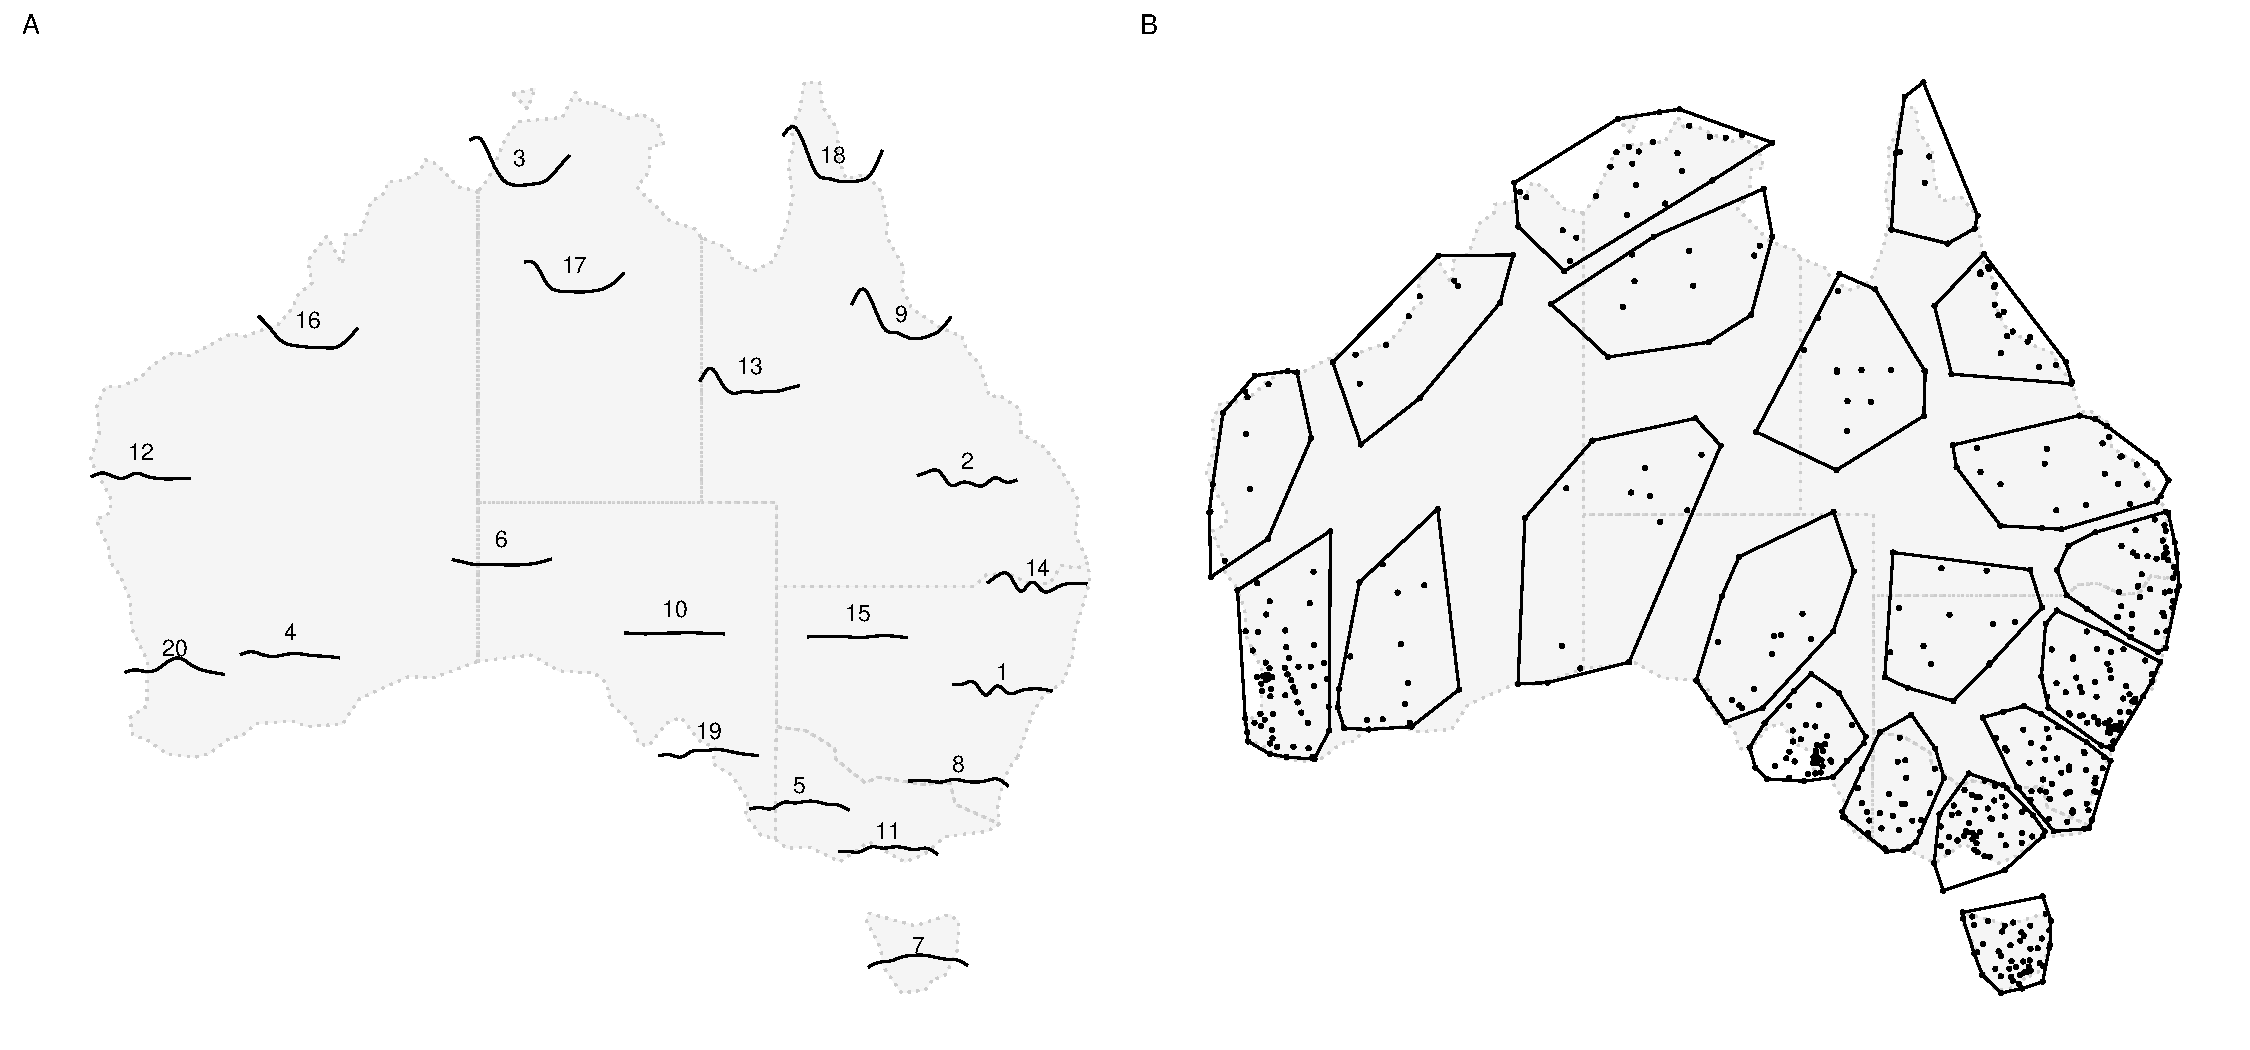
\includegraphics{figures/basic-agg-1} 

}

\caption[Profile of aggregated precipitation at 639 weather stations in Australia]{Profile of aggregated precipitation at 639 weather stations in Australia. Subplot A shows the glyph map of the weekly averaged precipitation of each cluster. The group number is printed in the middle of the y minor axis and can be used as a reference line to read the magnitude. Subplot B shows the station membership of each cluster.}\label{fig:basic-agg}
\end{figure}
\end{CodeChunk}

\hypertarget{river-level-data-in-victoria-water-gauges}{%
\subsection{River level data in Victoria water gauges}\label{river-level-data-in-victoria-water-gauges}}

The Bureau of Meteorology collects \href{http://www.bom.gov.au/metadata/catalogue/19115/ANZCW0503900528?template=full}{water data} from river gauges. The collected variables include: electrical conductivity, turbidity, watercourse discharge, watercourse level, and water temperature. We expect that the water level should be related to the precipitation available from climate data, since rainfall will raise the water level in the river. Figure \ref{fig:matching-map} shows the location of available weather stations and water gauges in Victoria, and we will try to match water gauges with nearby weather stations, taking into account both spatial and temporal information from 2020.

\begin{CodeChunk}
\begin{figure}

{\centering 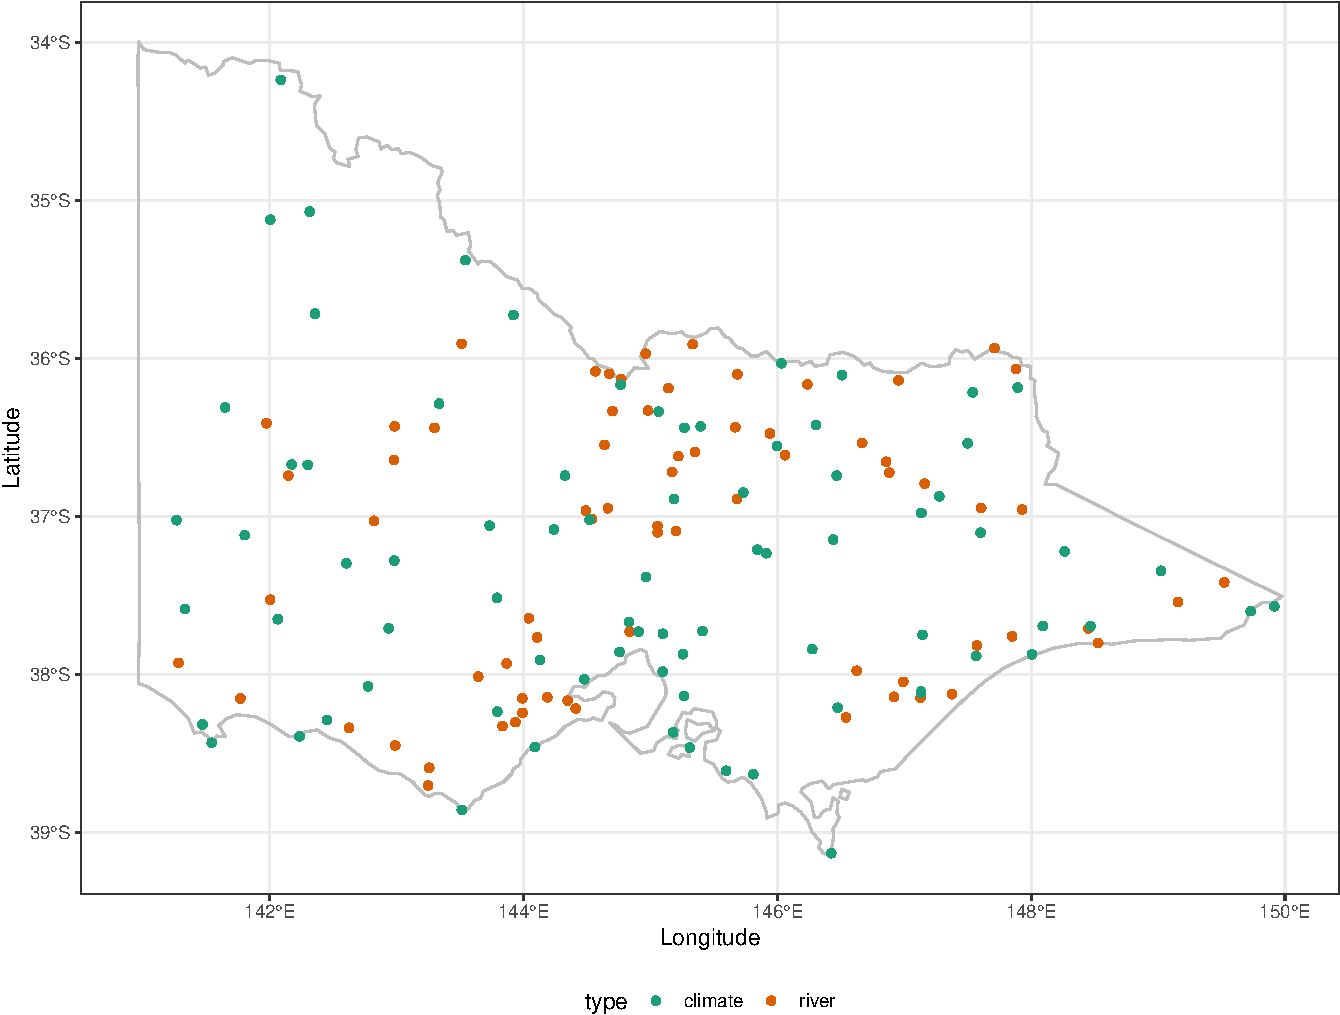
\includegraphics{figures/matching-map-1} 

}

\caption[Location of weather stations and river gauges in Victoria, Australia]{Location of weather stations and river gauges in Victoria, Australia.}\label{fig:matching-map}
\end{figure}
\end{CodeChunk}

As introduced in Section \ref{matching}, \code{match_sites()} can be used for this task, and we choose \code{Water_course_level} in \code{river} and \code{prcp} in \code{climate} for the temporal matching. We first pass in the two datasets, followed by the variables used for the temporal matching, specified in \code{temporal_by} (using the \code{by} syntax from \code{dplyr::join}). With \code{temporal_independent} we select precipitation (\code{prcp}) as the independent variable, and the goal is to see if the water level in the river reflects what is observed in precipitation (for nearby stations). Since we consider a full year of data, we set the number of peaks considered (\code{temporal_n_highest}) to 30 (slightly above the default value of 20), and \code{temporal_min_match} is raised accordingly.

\begin{CodeChunk}
\begin{CodeInput}
R> res <- match_sites(
+   river, climate,
+   temporal_by = c("Water_course_level" = "prcp"),
+   temporal_independent = "prcp",  
+   temporal_n_highest = 30,
+   temporal_min_match = 15
+ )
\end{CodeInput}
\end{CodeChunk}

The output from this function is also a cubble, with additional columns \code{dist} and \code{group} produced from spatial matching, and \code{n_match} from temporal matching.

\begin{CodeChunk}
\begin{CodeOutput}
# cubble:   id [8]: nested form
# bbox:     [144.52, -37.73, 146.06, -36.55]
# temporal: date [date], matched_var [dbl]
  id          name        lat  long type   dist group ts       n_match
  <chr>       <chr>     <dbl> <dbl> <chr> <dbl> <int> <list>     <int>
1 405234      SEVEN CR~ -36.9  146. river  6.15     5 <tibble>      21
2 404207      HOLLAND ~ -36.6  146. river  8.54    10 <tibble>      21
3 ASN00082042 strathbo~ -36.8  146. clim~  6.15     5 <tibble>      21
4 ASN00082170 benalla ~ -36.6  146. clim~  8.54    10 <tibble>      21
5 230200      MARIBYRN~ -37.7  145. river  6.17     6 <tibble>      19
# ... with 3 more rows
\end{CodeOutput}
\end{CodeChunk}

Figure \ref{fig:matching} (A) shows the four matched pairs on the map. For these the expected concurrent increase in precipitation and water level can be seen clearly when comparing these variables on a standardised scale, see Figure \ref{fig:matching} (B).

\begin{CodeChunk}
\begin{figure}

{\centering 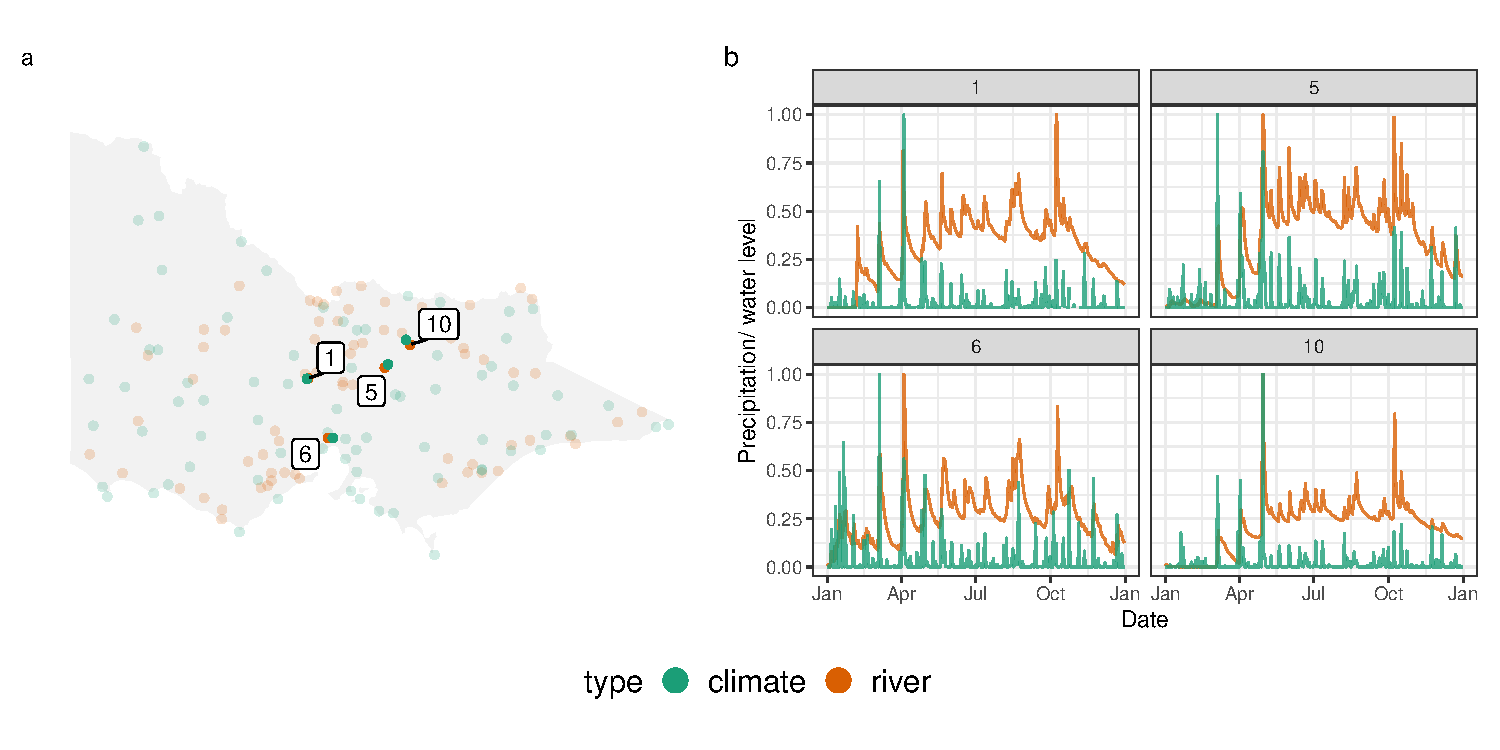
\includegraphics{figures/matching-1} 

}

\caption[Matched weather stations and river gauges on the map (A) and across time (B)]{Matched weather stations and river gauges on the map (A) and across time (B). Precipitation and water level have been standardised between 0 and 1 to be displayed on the same scale. The water level reflects the increase in precipitation. The numbers (1, 5, 6, 10) indicate the group index derived from spatial matching, only those that were selectd by temporal matching are shown here.}\label{fig:matching}
\end{figure}
\end{CodeChunk}

\hypertarget{era5-climate-reanalysis-data}{%
\subsection{ERA5: climate reanalysis data}\label{era5-climate-reanalysis-data}}

The ERA5 dataset \citep{hersbach2020era5} provides hourly estimates across the Earth for atmospheric, land and oceanic climate variables. The data is available in the NetCDF format from the European Centre for Medium-Range Weather Forecasts (ECMWF) and it can be directly downloaded from \href{https://cds.climate.copernicus.eu/cdsapp\#!/dataset/reanalysis-era5-pressure-levels?tab=overview}{Copernicus Climate Data Store (CDS)} website or programmatically via the R package \pkg{ecmwfr} \citep{ecwmfr}. In this example we focus on the \code{era5-pressure} data which provides hourly data on pressure levels from 1970 to present. Here we specifically look at the information contained on the variables \emph{specific humidity} measuring the mass of water vapor per kilogram of moist air and the \emph{geopotential} variable recording the gravitational potential energy of a unit mass, at a particular location, relative to mean sea level. The goal of this example is to reproduce the break-up of the southern polar vortex that happened in late September and early October in 2022 in the stratosphere in the Southern Hemisphere. Therefore, we filter data corresponding to the Southern Hemisphere and restrict our analysis to four dates: 2002-09-22, 2002-09-26, 2002-09-30, and 2002-10-04. Once downloaded, the data can be read into a \code{cubble} as:

\begin{CodeChunk}
\begin{CodeInput}
R> raw <- ncdf4::nc_open(here::here("data/era5-pressure.nc"))
R> dt <- as_cubble(raw, vars = c("q", "z"))
\end{CodeInput}
\end{CodeChunk}

Figure \ref{fig:netcdf} reproduces the ERA5 data row of Figure 19 in \citet{hersbach2020era5}. It shows the southern polar vortex splits into two on 2002-09-26 and further splits into four on 2002-10-04 in the stratosphere. Readers interested in the analysis of this figure can refer to \citet{hersbach2020era5}, \citet{simmons2020global}, and \citet{simmons2005ecmwf} for more details.

\begin{CodeChunk}
\begin{figure}

{\centering 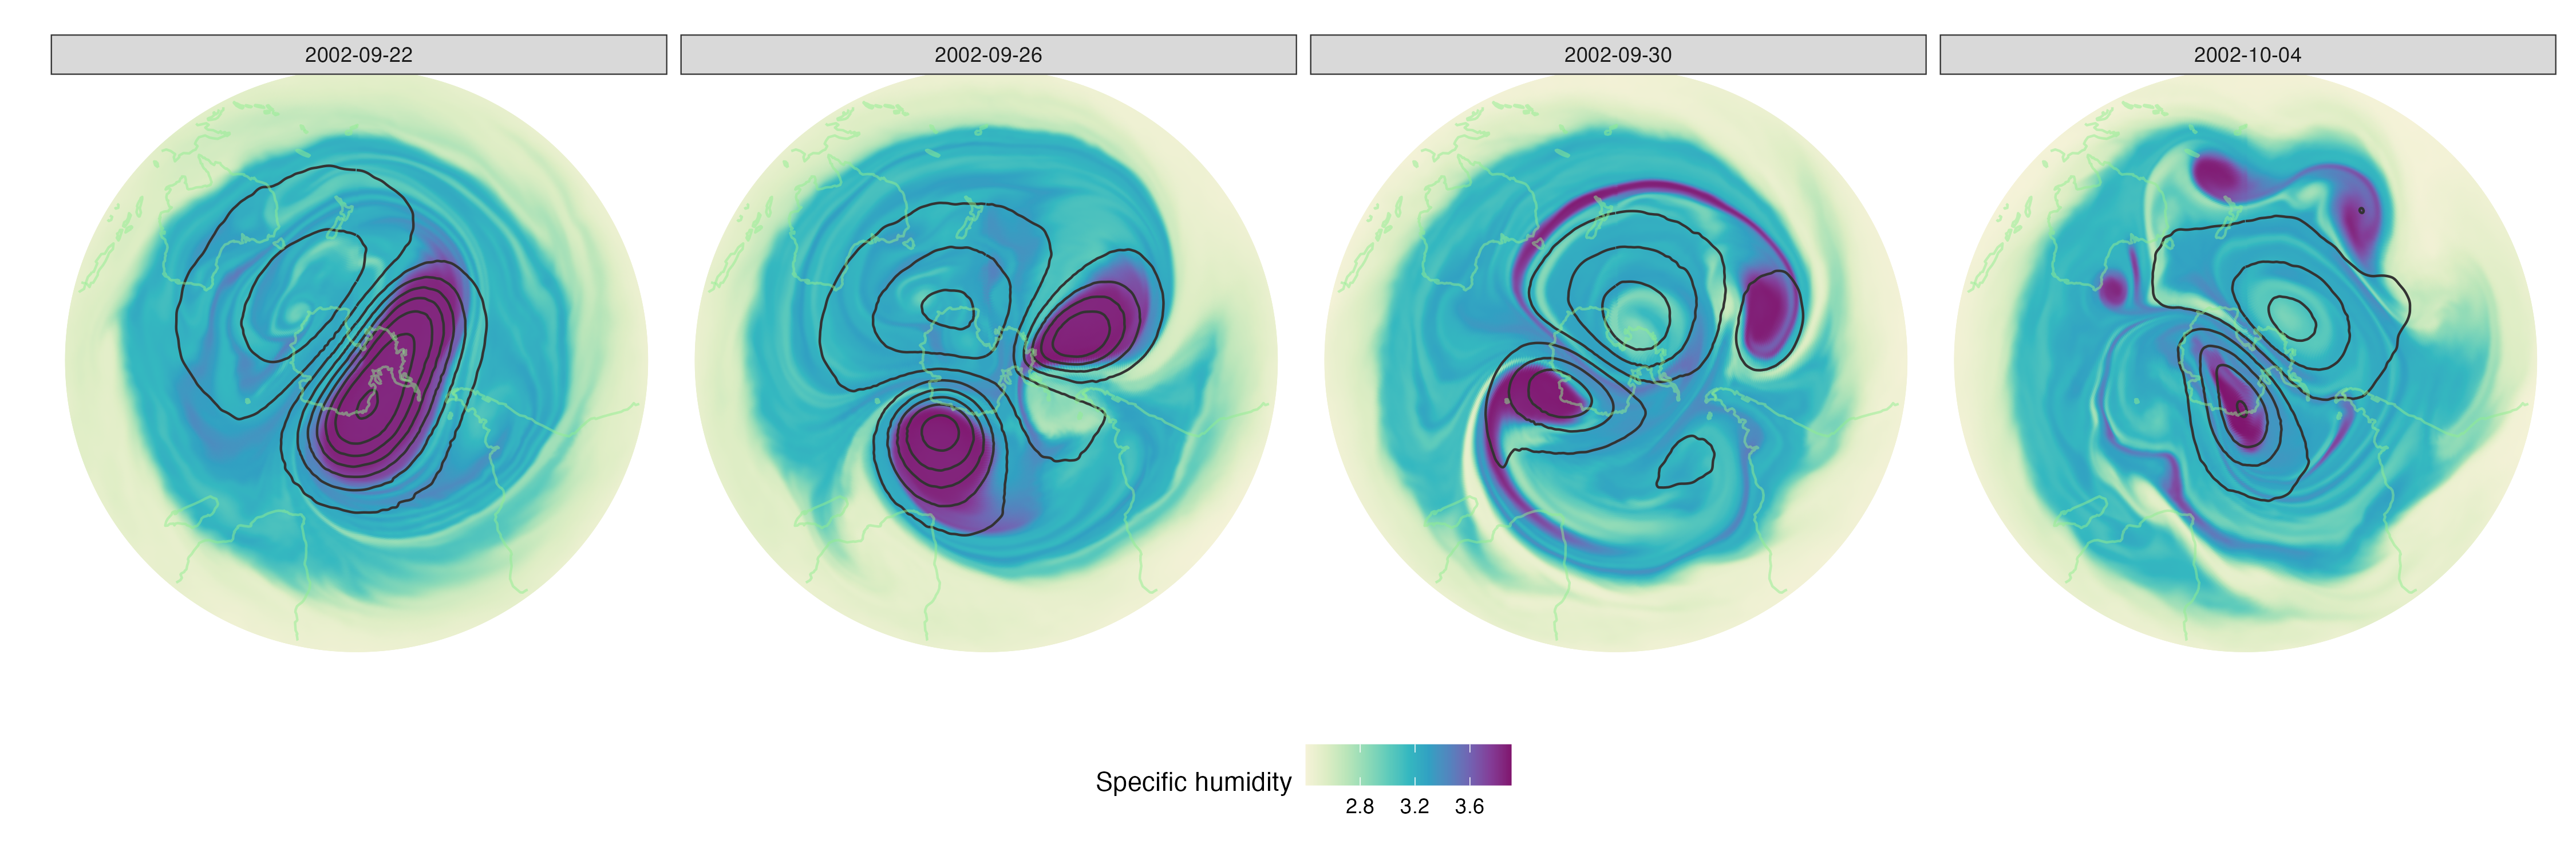
\includegraphics[width=1\linewidth]{../figures/netcdf} 

}

\caption[A reproduction of the second row (ERA5 data) of Figure 19 in Hersbach et al (2020)]{A reproduction of the second row (ERA5 data) of Figure 19 in Hersbach et al (2020).}\label{fig:netcdf}
\end{figure}
\end{CodeChunk}

\hypertarget{interactive-graphics-1}{%
\subsection{Interactive graphics}\label{interactive-graphics-1}}

When dealing with spatio-temporal data, users may wish to make plots to learn the spatial distribution of a variable or to find patterns, such as trend or seasonality, in the time series. Combining these two types of plots with interactivity lets users link between points on the map and the corresponding time series to explore the spatial and temporal dimensions of the data simultaneously. Below is an example that describes the process of building an interactive graphic with \pkg{cubble} and \pkg{crosstalk}. This example explores the variation of monthly temperature range within the \code{weatherdata::climate_full} data.

The temperature range is calculated as the difference between \code{tmax} and \code{tmin} and its monthly average over 2016-2020 is taken before calculating the variance. A \code{SharedData} object is constructed for each form of the cubble and the same \code{group} argument ensures the cross-linking of the two forms via the common \code{id} column. The spatial map and time series plot are then made with each \code{SharedData} object separately. In this example, stations on the Australia map, made from the nested form, are coloured by the calculated variance. A ribbon band is constructed using the long form cubble to show each station's maximum and minimum temperature over time. In the case of a different dataset, users could calculate other station-dependent measures in the nested form or make other time-wise summary of the data in the long form to customise the spatial or temporal view. The cross-linking between the two plots is always safeguarded by the shared \code{id} column embedded in the cubble structure. Below is the pseudo-code that outlines the process to construct the interactive graphic described above:

\begin{Shaded}
\begin{Highlighting}[]
\CommentTok{\# data pre{-}processing}
\NormalTok{clean }\OtherTok{\textless{}{-}}\NormalTok{ weatherdata}\SpecialCharTok{::}\NormalTok{climate\_full }\SpecialCharTok{|}\ErrorTok{\textgreater{}}\NormalTok{ ...}

\CommentTok{\# created SharedData instance for crosstalk}
\NormalTok{nested }\OtherTok{\textless{}{-}}\NormalTok{ clean }\SpecialCharTok{|}\ErrorTok{\textgreater{}}\NormalTok{ SharedData}\SpecialCharTok{$}\FunctionTok{new}\NormalTok{(}\SpecialCharTok{\textasciitilde{}}\NormalTok{id, }\AttributeTok{group =} \StringTok{"cubble"}\NormalTok{)}
\NormalTok{long }\OtherTok{\textless{}{-}} \FunctionTok{face\_temporal}\NormalTok{(clean) }\SpecialCharTok{|}\ErrorTok{\textgreater{}}\NormalTok{ SharedData}\SpecialCharTok{$}\FunctionTok{new}\NormalTok{(}\SpecialCharTok{\textasciitilde{}}\NormalTok{id, }\AttributeTok{group =} \StringTok{"cubble"}\NormalTok{)}

\CommentTok{\# create the spatial and temporal view each with a ShareData instance}
\NormalTok{p1 }\OtherTok{\textless{}{-}}\NormalTok{ nested }\SpecialCharTok{|}\ErrorTok{\textgreater{}}\NormalTok{ ...}
\NormalTok{p2 }\OtherTok{\textless{}{-}}\NormalTok{ long }\SpecialCharTok{|}\ErrorTok{\textgreater{}}\NormalTok{ ...}

\CommentTok{\# Combine p1 and p2}
\NormalTok{crosstalk}\SpecialCharTok{::}\FunctionTok{bscols}\NormalTok{(plotly}\SpecialCharTok{::}\FunctionTok{ggplotly}\NormalTok{(p1), plotly}\SpecialCharTok{::}\FunctionTok{ggplotly}\NormalTok{(p2), ...)}
\end{Highlighting}
\end{Shaded}

In Figure \ref{fig:interactive-linking}, the first row shows the initial view of the interactive graphic. Most regions in Australia have a low variance of temperature range, while the North-West coastline, the bottom of South Australia, and Victoria stand out with larger monthly changes. In the second row, the Mount Elizabeth station, which shows a high variance colour on the initial map, is selected on the map and this produces the ribbon on the right. In the third row, the lowest temperature in August is selected, which highlights the corresponding Thredbo AWS station on the left map. Another station in the Tasmania island is selected on the map to cross compare with Thredbo AWS.

\begin{CodeChunk}
\begin{figure}

{\centering 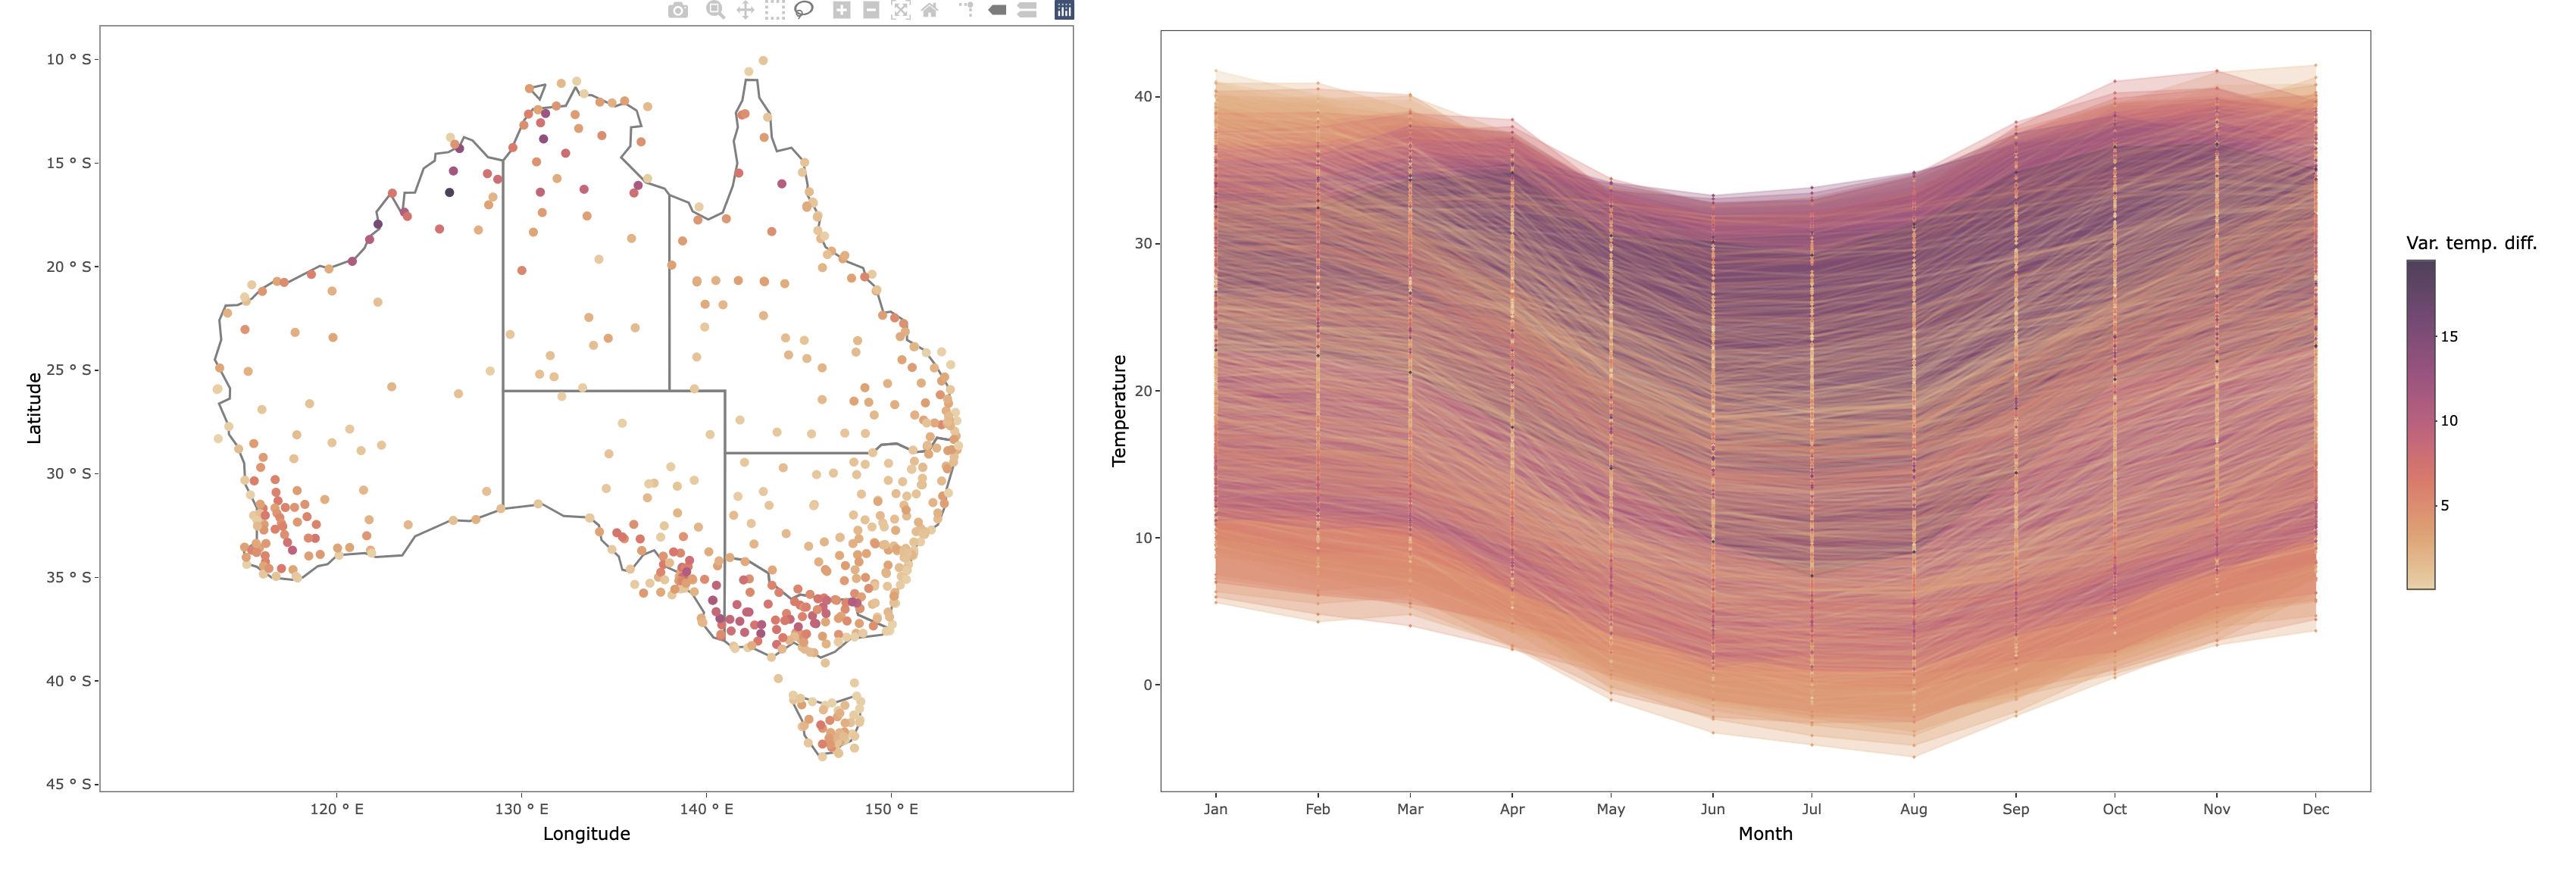
\includegraphics[width=1\linewidth,height=0.23\textheight]{../figures/linking} 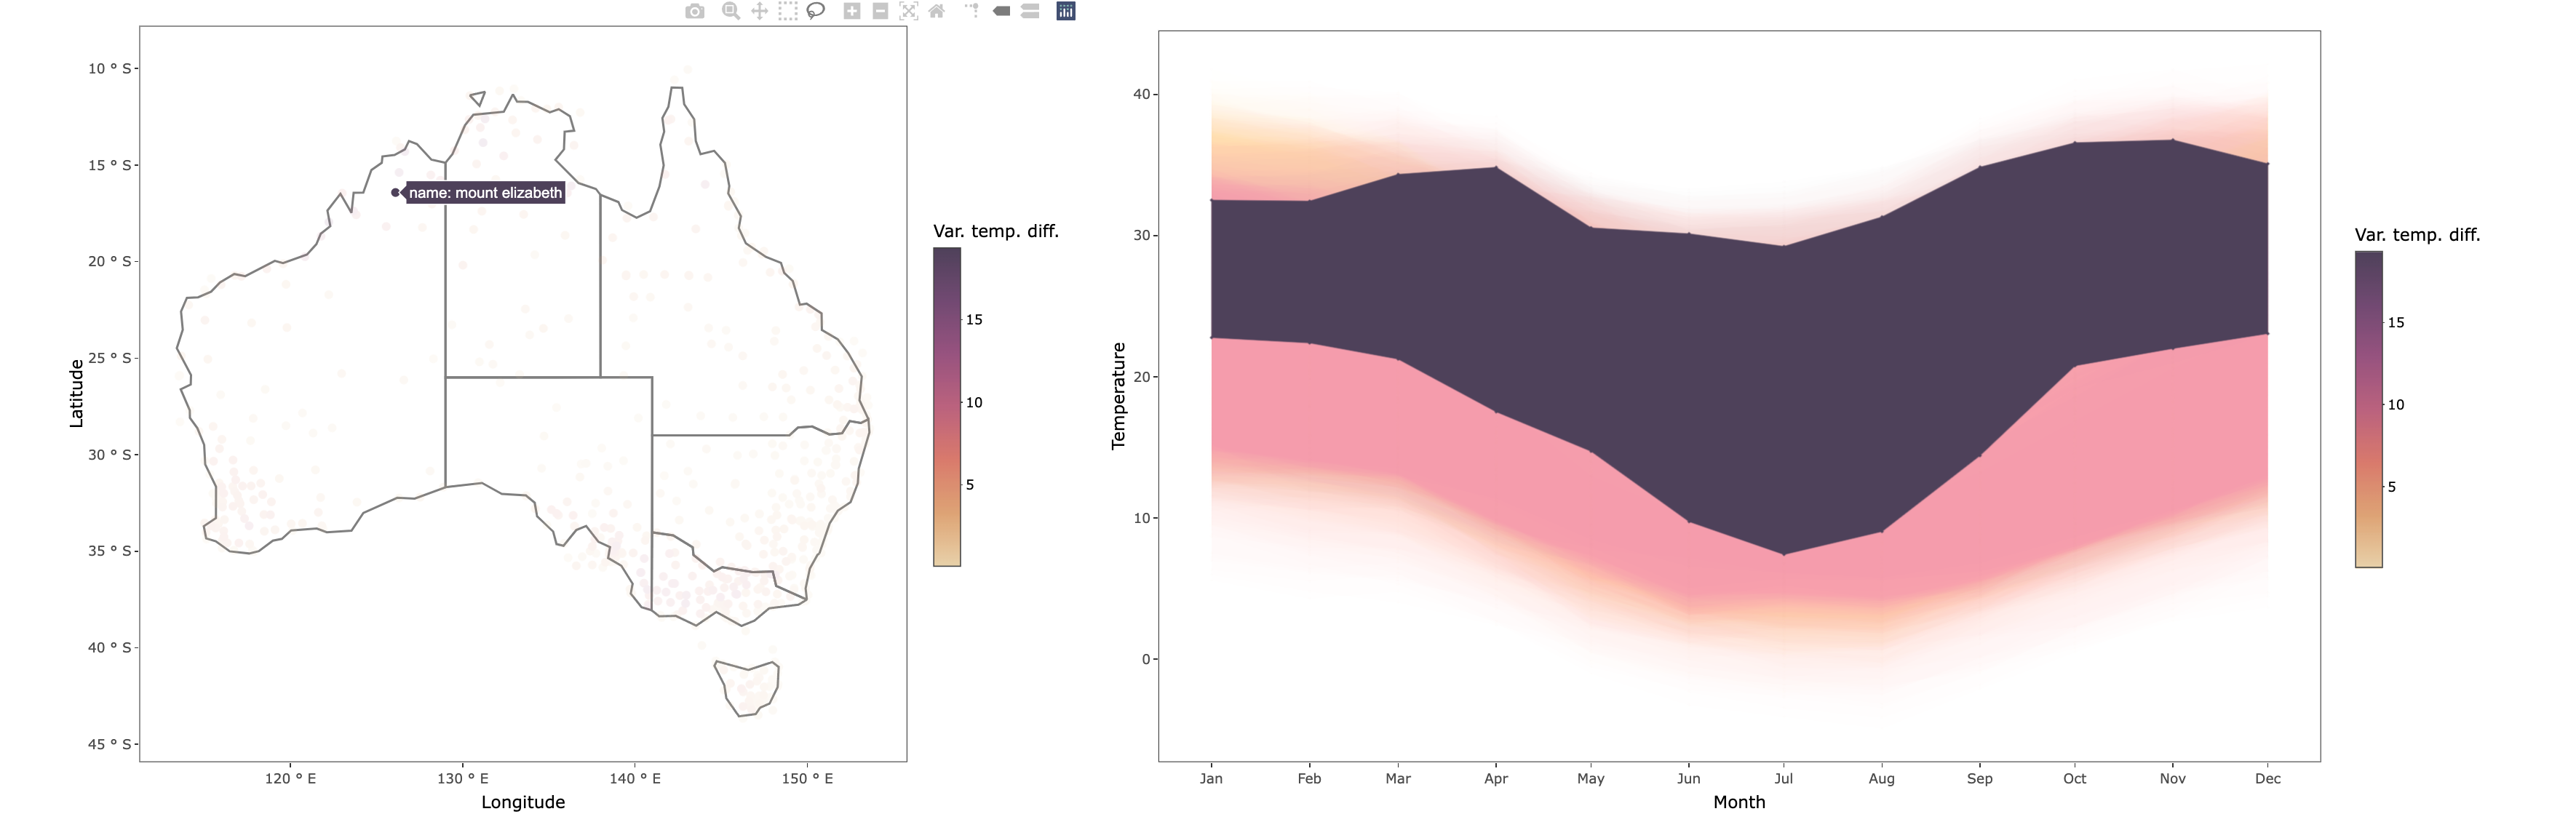
\includegraphics[width=1\linewidth,height=0.23\textheight]{../figures/linking-north} 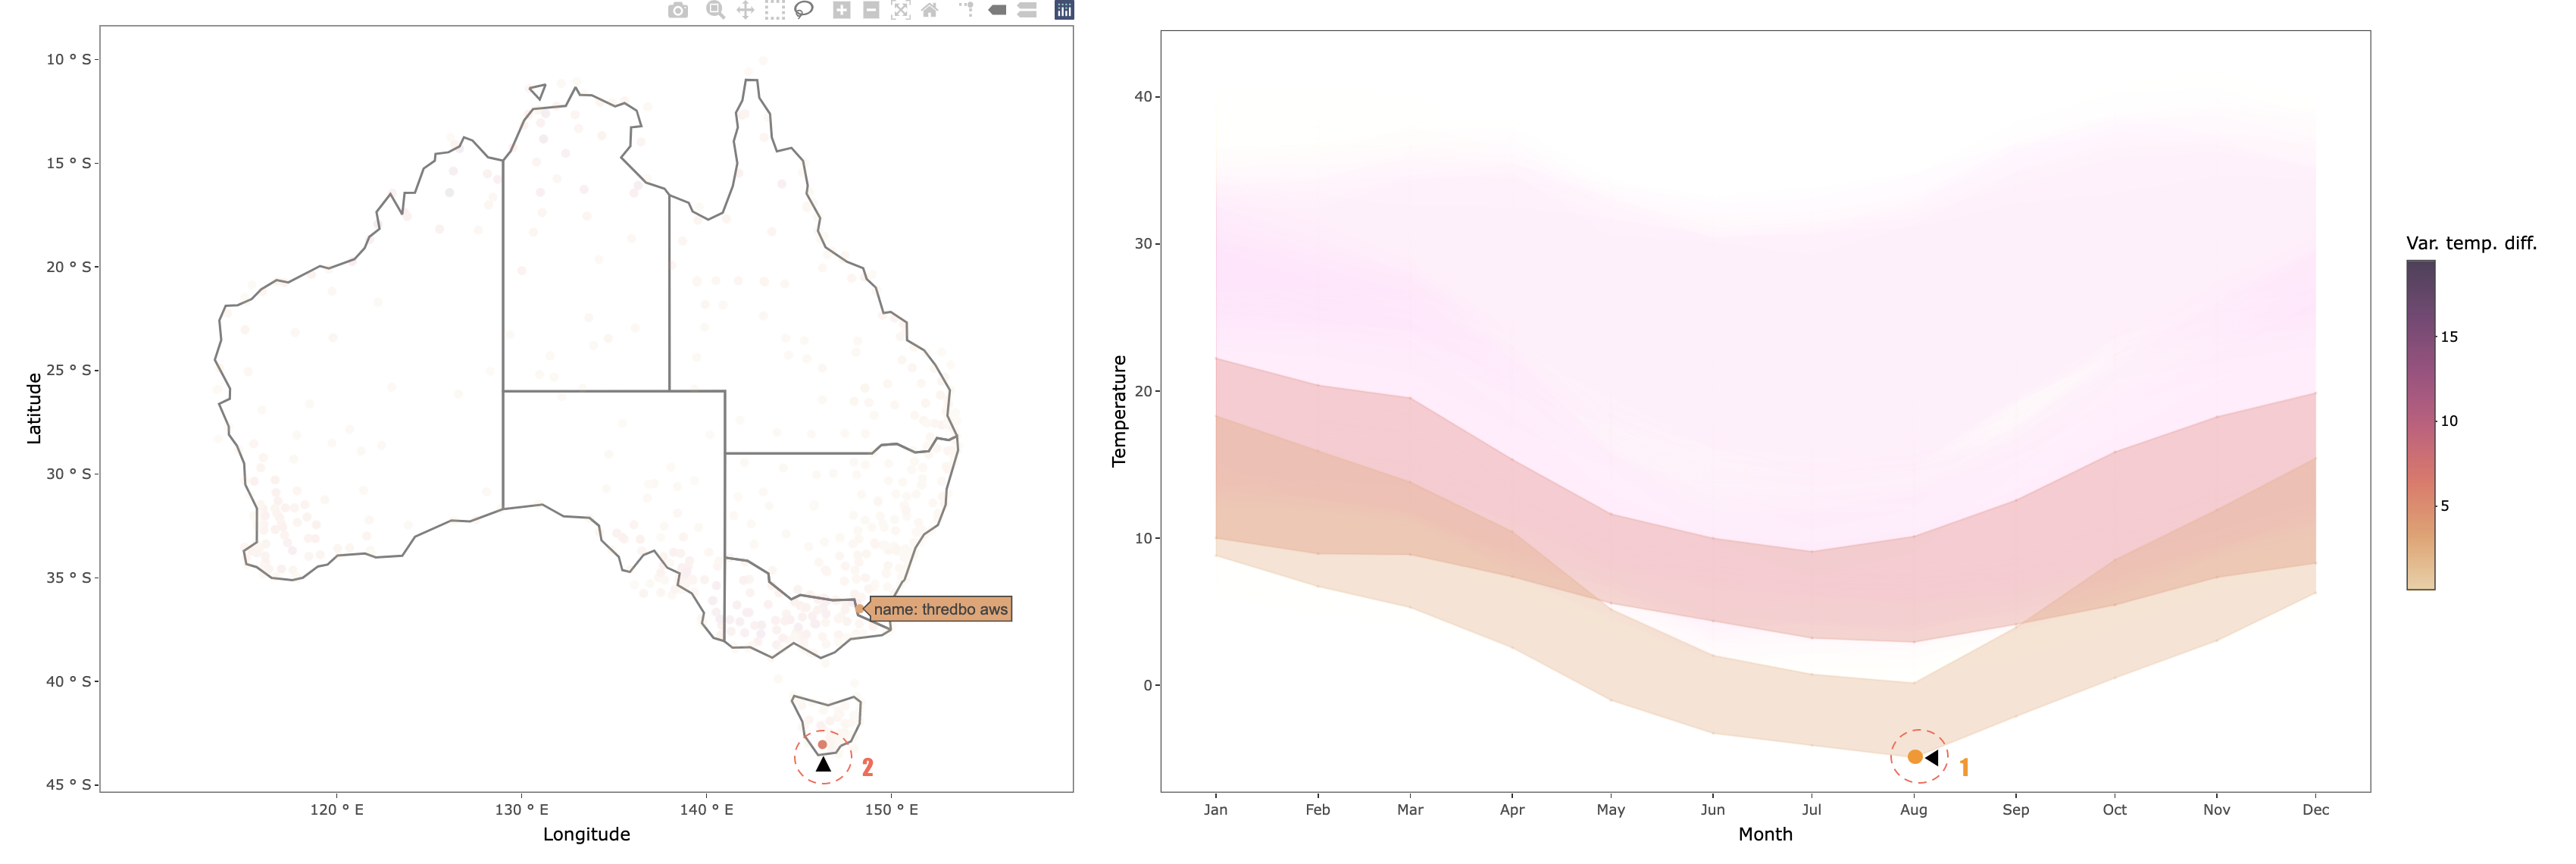
\includegraphics[width=1\linewidth,height=0.23\textheight]{../figures/linking-lower} 

}

\caption[Exploring temperature variation using linking of a map and seasonal display]{Exploring temperature variation using linking of a map and seasonal display. Each row is a screen dump of the process. The top row shows all locations and all temperature profiles. Selecting a particular location on the map (here Mount Elizabeth) produces the plot in the second row. The maximum and minimum temperatures are shown using a ribbon. The bottom row first selects the lowest temperature in August in the seasonal display, which highlights the corresponding station on the map (Thredbo AWS). Another  station, located in the Tasmania Island, is then selected to compare its temperature variation with Thredbo AWS.}\label{fig:interactive-linking}
\end{figure}
\end{CodeChunk}

This plot can also be made using \pkg{cubble} and \pkg{leaflet}, in which case the temperature range is displayed as a small subplot upon clicking on the map. This procedure involves first creating the popup plots from the long form cubble as a vector and then adding these plots to a leaflet map created from the nested cubble, with \code{leafpop::addPopupGraphs()}:

\begin{Shaded}
\begin{Highlighting}[]
\CommentTok{\# data pre{-}processing}
\NormalTok{clean }\OtherTok{\textless{}{-}}\NormalTok{ weatherdata}\SpecialCharTok{::}\NormalTok{climate\_full }\SpecialCharTok{|}\ErrorTok{\textgreater{}}\NormalTok{ ...}

\CommentTok{\# use the long form to create subplots for each station}
\NormalTok{df\_id }\OtherTok{\textless{}{-}} \FunctionTok{unique}\NormalTok{(clean}\SpecialCharTok{$}\NormalTok{id)}
\NormalTok{p }\OtherTok{\textless{}{-}} \FunctionTok{map}\NormalTok{(}\DecValTok{1}\SpecialCharTok{:}\FunctionTok{length}\NormalTok{(df\_id), }\ControlFlowTok{function}\NormalTok{(i)\{}
\NormalTok{  dt }\OtherTok{\textless{}{-}}\NormalTok{ clean }\SpecialCharTok{|}\ErrorTok{\textgreater{}} \FunctionTok{filter}\NormalTok{(id }\SpecialCharTok{==}\NormalTok{ df\_id[i])}
  \FunctionTok{ggplot}\NormalTok{(dt) }\SpecialCharTok{|}\ErrorTok{\textgreater{}}\NormalTok{ ...}
\NormalTok{\})}

\CommentTok{\# create nested form leaflet map with temperature band as subplots}
\NormalTok{nested }\OtherTok{\textless{}{-}} \FunctionTok{face\_spatial}\NormalTok{(clean)}
\FunctionTok{leaflet}\NormalTok{(nested) }\SpecialCharTok{|}\ErrorTok{\textgreater{}}
  \FunctionTok{addTiles}\NormalTok{() }\SpecialCharTok{|}\ErrorTok{\textgreater{}}
  \FunctionTok{addCircleMarkers}\NormalTok{(}\AttributeTok{group =} \StringTok{"a"}\NormalTok{, ...) }\SpecialCharTok{|}\ErrorTok{\textgreater{}}
\NormalTok{  leafpop}\SpecialCharTok{::}\FunctionTok{addPopupGraphs}\NormalTok{(}\AttributeTok{graph =}\NormalTok{ p, ...)}
\end{Highlighting}
\end{Shaded}

Figure \ref{fig:interactive-popup} shows the same information as Figure \ref{fig:interactive-linking} but using leaflet and popups \citep{leafpop}.

\begin{CodeChunk}
\begin{figure}

{\centering 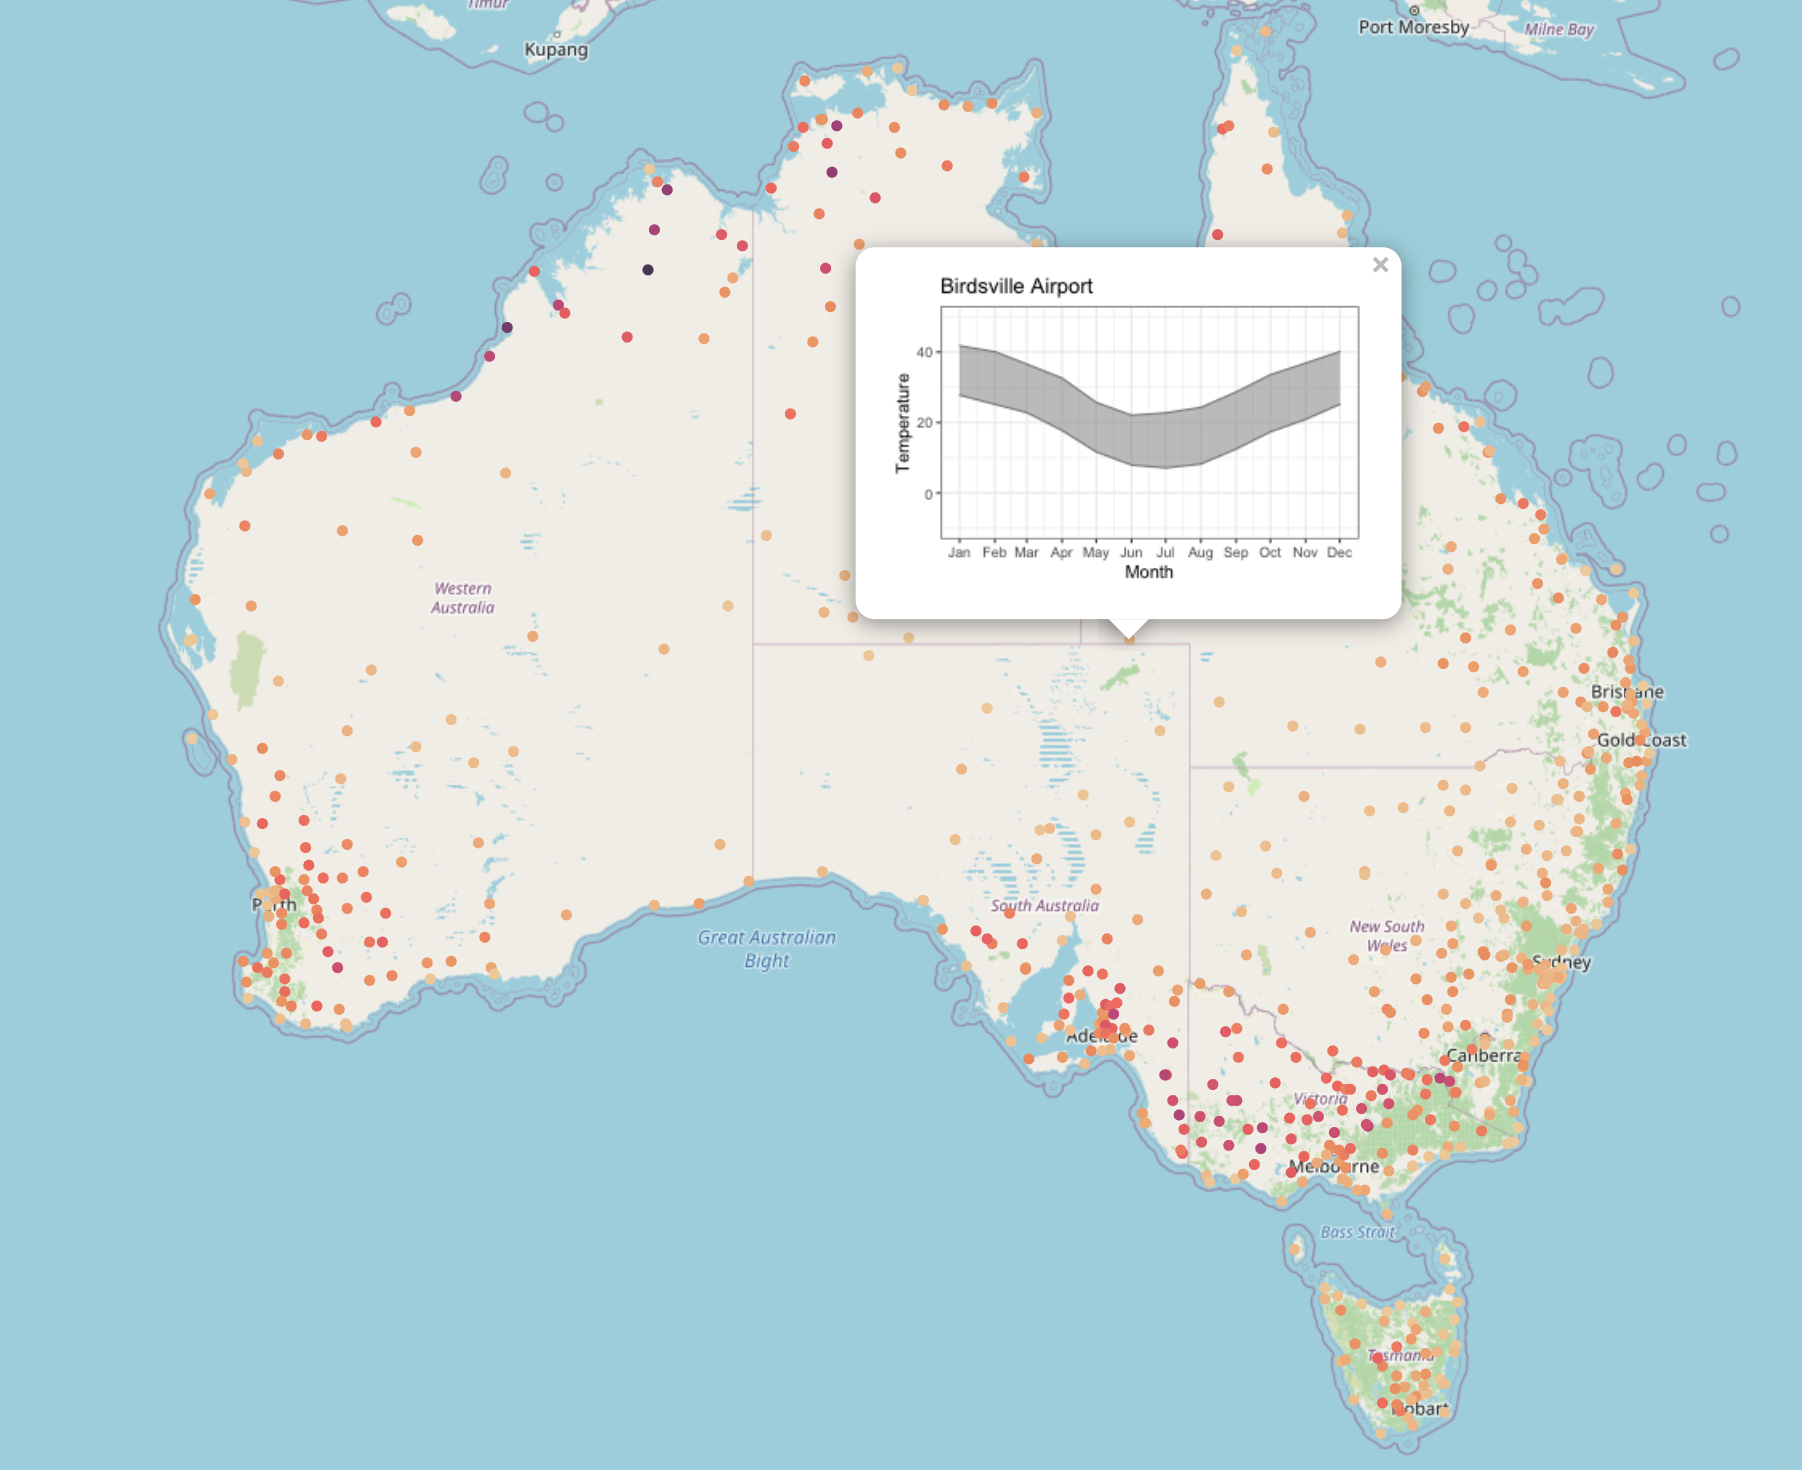
\includegraphics[width=0.45\linewidth,height=0.25\textheight]{../figures/popup-mid} 

}

\caption[Same as Figure 11 except the temperature variation is now shown as a popup in the leaflet map]{Same as Figure 11 except the temperature variation is now shown as a popup in the leaflet map.}\label{fig:interactive-popup}
\end{figure}
\end{CodeChunk}

\hypertarget{conclude}{%
\section{Conclusion}\label{conclude}}

This paper presents an \proglang{R} package \pkg{cubble} for organising, manipulating and visualising spatio-temporal data. The package introduces a new data structure for spatio-temporal data, \code{cubble}, that connects the time invariant and varying variables and that allows the user to work with a nested and long form of the data. TThe goal of this work is to add capabilities into the spatio-temporal practitioners toolbox that facilitates their work within the tidy data framework. The data structure and the capabilities introduced in this package can be used and combined with existing spatio-temporal R packages such as \pkg{sf}, data wrangling packages such as \pkg{dplyr}, and visualization packages such as \pkg{ggplot2}, \pkg{plotly} and \pkg{leaflet}.

The data structure and functions are demonstrated with extensive examples. These include creating and coercing wild-caught data with potential mismatch on sites, handling hierarchical data, matching time series spatially and temporally, as well as reproducing ERA5 results from NetCDF data. Visualization of the \code{cubble} objects and derivatives is presented via interactive graphic pipelines using \pkg{plotly} and \pkg{leaflet}.

Future directions of the package involves handling sites with moving coordinates. This would involve constructing a list-column for location coordinates and a form these locations can be pivoted into, like the long form for temporal variables. In the multivariate aspect, \pkg{cubble} can also be extended with interface to more high dimensional visualisation methods, i.e., the tour method, to understand variable importance or comparing location similarities.

\newpage

\hypertarget{acknowledgement}{%
\section{Acknowledgement}\label{acknowledgement}}

This work is funded by a Commonwealth Scientific and Industrial Research Organisation (CSIRO) Data61 Scholarship and started while Nicolas Langrené was affiliated with CSIRO's Data61. The article is created using \pkg{knitr} \citep{knitr} and \pkg{rmarkdown} \citep{rmarkdown} in R. The source code for reproducing this paper can be found at: \url{https://github.com/huizezhang-sherry/paper-cubble}.

\bibliography{../references.bib}



\end{document}
